% ============================================================
%  يُترجَم بـ XeLaTeX  (في Overleaf: Menu → Compiler → XeLaTeX)
%  الخط: Amiri (متوفر في Overleaf، أو حمّله من github.com/aliftype/amiri)
% ============================================================
\documentclass[12pt,a4paper]{article}
\usepackage[a4paper,margin=1.7cm,top=2.3cm,bottom=2.9cm,headheight=15pt,footskip=1.5cm]{geometry}
\usepackage{amsmath,amssymb}
\usepackage{icomma}
\usepackage[english,bidi=default,layout=lists]{babel}
\babelprovide[import,main]{arabic}
\babelfont{rm}[Scale=1.08]{Amiri}
\babelfont{sf}[Scale=1.08]{Amiri}
\usepackage[most]{tcolorbox}
\usepackage{tikz}
\usetikzlibrary{arrows.meta,calc,shadings,patterns}
\usepackage{array}
\usepackage{colortbl}
\usepackage{fancyhdr}
\usepackage{titlesec}
\usepackage{enumitem}
\usepackage{collcell}
\usepackage{needspace}
\usepackage{etoolbox}
\newcolumntype{C}{>{\collectcell\ar}c<{\endcollectcell}}
\pretocmd{\section}{\Needspace{15\baselineskip}}{}{}
\pretocmd{\subsection}{\Needspace{11\baselineskip}}{}{}

\definecolor{cDef}{HTML}{1F4E9C}
\definecolor{cThm}{HTML}{B3261E}
\definecolor{cRem}{HTML}{2E7D32}
\definecolor{cEx}{HTML}{C76B00}
\definecolor{cMeth}{HTML}{6A1B9A}
\definecolor{cSol}{HTML}{00695C}
\definecolor{cSec}{HTML}{1F3A68}

\titleformat{\section}{\Large\bfseries\color{cSec}}{\thesection.}{0.6em}{}[{\color{cSec!60}\titlerule[1pt]}]
\titleformat{\subsection}{\large\bfseries\color{cThm!85!black}}{\thesubsection.}{0.5em}{}
\titlespacing*{\section}{0pt}{14pt}{8pt}
\titlespacing*{\subsection}{0pt}{10pt}{5pt}
\setlength{\parindent}{0pt}
\setlength{\parskip}{4pt}
\setlist{itemsep=2pt,topsep=3pt}

\newtcolorbox{arbox}[3][]{enhanced,
  colback=#2!5,colframe=#2!80!black,arc=2mm,boxrule=0.8pt,
  left=6pt,right=6pt,top=8pt,bottom=5pt,
  fonttitle=\bfseries,coltitle=white,
  title={\foreignlanguage{arabic}{#3}},
  attach boxed title to top right={xshift=-5mm,yshift=-3mm},
  boxed title style={colback=#2!80!black,arc=1.5mm,boxrule=0pt},
  before upper={\selectlanguage{arabic}},
  before skip=8pt,after skip=8pt,breakable,#1}
\newenvironment{BOX}[2]{\begin{otherlanguage}{english}\begin{arbox}{#1}{#2}}{\end{arbox}\end{otherlanguage}}
\newenvironment{tarif}[1][تعريف]{\begin{BOX}{cDef}{#1}}{\end{BOX}}
\newenvironment{khassia}[1][خاصية]{\begin{BOX}{cThm}{#1}}{\end{BOX}}
\newenvironment{molahada}[1][ملاحظة]{\begin{BOX}{cRem}{#1}}{\end{BOX}}
\newenvironment{mithal}[1][مثال]{\begin{BOX}{cEx}{#1}}{\end{BOX}}
\newenvironment{tariqa}[1][طريقة]{\begin{BOX}{cMeth}{#1}}{\end{BOX}}

\newcounter{exo}
\newenvironment{tamrin}[1]{\stepcounter{exo}\begin{BOX}{cSec}{التمرين \theexo: #1}}{\end{BOX}}
\newenvironment{hal}{\Needspace{12\baselineskip}\begin{otherlanguage}{english}\begin{arbox}[breakable]{cSol}{حل التمرين \theexo}}{\end{arbox}\end{otherlanguage}}

\newenvironment{LTR}{\begin{otherlanguage}{english}}{\end{otherlanguage}}
\newcommand{\ar}[1]{\foreignlanguage{arabic}{#1}}

\renewcommand{\dots}{\mathinner{\ldotp\ldotp\ldotp}}
\renewcommand{\ldots}{\mathinner{\ldotp\ldotp\ldotp}}
\renewcommand{\cdots}{\mathinner{\cdotp\cdotp\cdotp}}
\newcommand{\N}{\mathbb{N}}
\newcommand{\Z}{\mathbb{Z}}
\newcommand{\D}{\mathbb{D}}
\newcommand{\Q}{\mathbb{Q}}
\newcommand{\R}{\mathbb{R}}
\newcommand{\pgcd}{\operatorname{PGCD}}
\newcommand{\ppcm}{\operatorname{PPCM}}

% \NLseg{a}{b}{[}{]} ; \NLright{a}{[} ; \NLleft{b}{]}  (interval on a number line)
\newcommand{\NLseg}[4]{\begin{LTR}\begin{tikzpicture}[baseline=-0.6ex]
 \draw[-{Stealth[length=2mm]},gray!70](0,0)--(3.4,0);
 \draw[line width=2pt,cThm!80!black](0.7,0)--(2.7,0);
 \node[cThm!80!black,font=\LARGE] at (0.7,0){$#3$};
 \node[cThm!80!black,font=\LARGE] at (2.7,0){$#4$};
 \node[below=3pt,font=\footnotesize] at (0.7,0){$#1$};
 \node[below=3pt,font=\footnotesize] at (2.7,0){$#2$};
\end{tikzpicture}\end{LTR}}
\newcommand{\NLright}[2]{\begin{LTR}\begin{tikzpicture}[baseline=-0.6ex]
 \draw[-{Stealth[length=2mm]},gray!70](0,0)--(3.4,0);
 \draw[line width=2pt,cThm!80!black](1.3,0)--(3.3,0);
 \node[cThm!80!black,font=\LARGE] at (1.3,0){$#2$};
 \node[below=3pt,font=\footnotesize] at (1.3,0){$#1$};
\end{tikzpicture}\end{LTR}}
\newcommand{\NLleft}[2]{\begin{LTR}\begin{tikzpicture}[baseline=-0.6ex]
 \draw[-{Stealth[length=2mm]},gray!70](0,0)--(3.4,0);
 \draw[line width=2pt,cThm!80!black](0.05,0)--(2.1,0);
 \node[cThm!80!black,font=\LARGE] at (2.1,0){$#2$};
 \node[below=3pt,font=\footnotesize] at (2.1,0){$#1$};
\end{tikzpicture}\end{LTR}}

% ---------- social-media icons (pure TikZ) ----------
\definecolor{cFB}{HTML}{1877F2}
\definecolor{cTG}{HTML}{229ED9}
\definecolor{cIG1}{HTML}{FEDA75}
\definecolor{cIG2}{HTML}{D62976}
\definecolor{cIG3}{HTML}{4F5BD5}
\newcommand{\fbicon}{\begin{LTR}\begin{tikzpicture}[baseline=-0.75ex,x=1em,y=1em]
 \fill[cFB] (0,0) circle (0.55);
 \node[white,inner sep=0,font=\usefont{TU}{lmss}{bx}{n}\small] at (0.04,-0.02) {f};
\end{tikzpicture}\end{LTR}}
\newcommand{\igicon}{\begin{LTR}
\begin{tikzpicture}[baseline=-0.75ex,x=1em,y=1em]
 \shade[lower left=cIG1,lower right=cIG2,upper left=cIG2,upper right=cIG3,rounded corners=0.28em] (-0.55,-0.55) rectangle (0.55,0.55);
 \draw[white,line width=0.09em,rounded corners=0.18em] (-0.36,-0.36) rectangle (0.36,0.36);
 \draw[white,line width=0.09em] (0,0) circle (0.17);
 \fill[white] (0.22,0.22) circle (0.05);
\end{tikzpicture}\end{LTR}}
\newcommand{\tgicon}{\begin{LTR}
\begin{tikzpicture}[baseline=-0.75ex,x=1em,y=1em]
 \fill[cTG] (0,0) circle (0.55);
 \fill[white] (-0.33,0.0) -- (0.32,0.27) -- (0.2,-0.3) -- (0.0,-0.15) -- (-0.08,-0.28) -- (-0.08,-0.08) -- cycle;
 \fill[cTG!70!black] (-0.08,-0.08) -- (0.25,0.2) -- (0.0,-0.15) -- (-0.08,-0.28) -- cycle;
\end{tikzpicture}\end{LTR}}
% page number: black box, white two-digit number, at the right of the social row
\newcommand{\PageBox}{\begin{LTR}\tikz[baseline=(p.base)]\node[fill=black,text=white,inner sep=2.5pt,minimum width=1.6em,minimum height=1.3em,font=\usefont{TU}{lmss}{bx}{n}\small](p){\ifnum\value{page}<10 0\fi\arabic{page}};\end{LTR}}
% visual left-to-right order: Telegram | Instagram | Facebook | page box
\newcommand{\SocialRow}{\begin{otherlanguage}{english}%
 \ar{\textbf{الأستاذ سوايسية هشام للرياضيات}}\ \tgicon\hfill
 \textbf{prof\_hicham\_math}\ \igicon\hfill
 \ar{\textbf{الأستاذ سوايسية هشام للرياضيات}}\ \fbicon\hspace{2.2em}\PageBox\end{otherlanguage}}

\pagestyle{fancy}
\fancyhf{}
\renewcommand{\headrulewidth}{0.6pt}
\renewcommand{\footrulewidth}{0.4pt}
% \SetHeader{right head: document title}{left head: level -- stream}
\newcommand{\SetHeader}[2]{%
 \fancyhead[C]{\parbox{\textwidth}{\ar{#1\hfill #2}}}%
 \fancyfoot[C]{\parbox{\textwidth}{\small\SocialRow}}}
\usepackage{tkz-tab}
\usepackage{multicol}
% variation / sign table (LTR)
\newenvironment{TAB}{\par\begin{center}\begin{LTR}\begin{tikzpicture}[scale=0.95,every node/.style={font=\small}]}{\end{tikzpicture}\end{LTR}\end{center}}
% grid + axes, clipped: \begin{GR}{xmin}{xmax}{ymin}{ymax}{unit cm}
\newenvironment{GR}[5]{\par\begin{center}\begin{LTR}\begin{tikzpicture}[x=#5cm,y=#5cm,font=\footnotesize]
 \draw[gray!25,very thin] (#1,#3) grid (#2,#4);
 \draw[-{Stealth[length=2mm]}] (#1,0)--(#2+0.3,0) node[below left]{$x$};
 \draw[-{Stealth[length=2mm]}] (0,#3)--(0,#4+0.3) node[below left]{$y$};
 \node[below left] at (0,0){$O$};
 \begin{scope}\clip (#1,#3) rectangle (#2,#4);}
{\end{scope}\end{tikzpicture}\end{LTR}\end{center}}
\newcommand{\Ticks}[2]{\foreach \t in {#1} \node[below,font=\scriptsize] at (\t,0){$\t$}; \foreach \t in {#2} \node[left,font=\scriptsize] at (0,\t){$\t$};}
\newcommand{\bx}[1]{\ensuremath{\colorbox{cDef!12}{$\displaystyle #1$}}}
\newcommand{\TwoCol}[4]{\par\begin{LTR}\noindent\begin{minipage}[t]{#1\textwidth}\selectlanguage{arabic}#2\end{minipage}\hfill\begin{minipage}[t]{#3\textwidth}\selectlanguage{arabic}#4\end{minipage}\end{LTR}\par}
\newcommand{\RL}[4]{\TwoCol{#3}{#4}{#1}{#2}}  % \RL{w1}{right content}{w2}{left content}
\newcommand{\ok}{$\textcolor{cRem}{\checkmark}$}
\newcommand{\limn}{\displaystyle\lim_{n\to+\infty}}
% sub-questions, each on its own line
\newenvironment{sq}{\begin{itemize}[leftmargin=2.4em,itemsep=3pt]}{\end{itemize}}
\newcommand{\qa}{\item[(أ)]}\newcommand{\qb}{\item[(ب)]}\newcommand{\qc}{\item[(جـ)]}\newcommand{\qd}{\item[(د)]}\newcommand{\qe}{\item[(هـ)]}
\newcommand{\pa}{\par\smallskip\textbf{(أ)} }\newcommand{\pb}{\par\smallskip\textbf{(ب)} }\newcommand{\pc}{\par\smallskip\textbf{(جـ)} }\newcommand{\pd}{\par\smallskip\textbf{(د)} }\newcommand{\pe}{\par\smallskip\textbf{(هـ)} }
\newcommand{\QQ}[1]{\par\smallskip\textbf{#1.} }
\newenvironment{tmr}{\stepcounter{exo}\begin{BOX}{cSec}{تمرين محلول \theexo}}{\end{BOX}}
\newcommand{\ABC}[3]{\\[2pt]\begin{tabular}{p{0.28\textwidth}p{0.28\textwidth}p{0.28\textwidth}}(جـ) \ #3 & (ب) \ #2 & (أ) \ #1\end{tabular}}
\newtcbox{\bxtbox}{on line,colback=cDef!12,colframe=cDef!12,boxrule=0pt,arc=1pt,boxsep=0pt,left=2pt,right=2pt,top=1pt,bottom=1pt}
\newcommand{\bxt}[1]{\foreignlanguage{english}{\bxtbox{\ar{#1}}}}
\SetHeader{\small\bfseries\color{cSec}تمارين الدالة الأسية}{\small\color{cSec}السنة الثالثة ثانوي -- تسيير واقتصاد}
\newenvironment{FIG}{\par\begin{center}\begin{LTR}}{\end{LTR}\end{center}}
\renewcommand{\bx}[1]{\ensuremath{\colorbox{cDef!12}{$\displaystyle\color{cThm}#1$}}}
\newcommand{\LW}[1]{{\color{cDef}#1}}
\newcommand{\Car}[1]{\left\{\begin{array}{l}#1\end{array}\right.}
\newcommand{\Lm}[1]{\displaystyle\lim_{x\to#1}}
\newcommand{\LD}[3]{\par لدينا: $\Lm{#2}#1=\bx{#3}$ لأنّ: \quad}
\newcommand{\E}{\par\smallskip}
\relpenalty=10000\binoppenalty=10000\tolerance=9000\emergencystretch=0.3\linewidth
\begin{document}
\begin{LTR}
\begin{tcolorbox}[enhanced,colback=cSec,colframe=cSec,arc=3mm,halign=center,boxrule=0pt,top=12pt,bottom=12pt,before upper={\selectlanguage{arabic}}]
{\color{white}\fontsize{28}{34}\selectfont\bfseries تمارين الدالة الأسية}\\[8pt]
{\color{white}\large تمارين من الاختبارات + مسائل البكالوريا (2017 -- 2026) + اختيار من متعدد ، مع الحلول المفصلة}\\[5pt]
{\color{white}\large السنة الثالثة ثانوي -- شعبة تسيير واقتصاد}
\end{tcolorbox}
\end{LTR}

\begin{molahada}
\begin{itemize}
\item الأسئلة المشار إليها بـ $(\star)$ تتطلب درس الدالة الأصلية والحساب التكاملي ، ويمكن تأجيلها إلى ما بعد دراسته.
\item الدالة اللوغاريتمية مدروسة قبل الدالة الأسية في شعبة تسيير واقتصاد ، فيمكن استعمالها في كل الأسئلة.
\item النهايات مكتوبة على الشكل: «لدينا: النهاية $=$ النتيجة لأنّ:» ثم النهايات الجزئية في حاضنة.
\end{itemize}
\end{molahada}

% =====================================================
\section{تمارين من الاختبارات (البكالوريا التجريبية)}

\begin{tamrin}{بكالوريا تجريبية 2026 -- تسيير واقتصاد (وهران) -- التمرين الثالث}
$P(x)$ كثير الحدود المعرف على $\R$ بـ: $P(x)=2x^3-6x-4$.
\QQ{1}
\begin{sq}
\qa تحقق أنه من أجل كل عدد حقيقي $x$: $P(x)=(2x-4)(x+1)^2$.
\qb حل في $\R$ المعادلة $P(x)=0$.
\end{sq}
\QQ{2} اعتمادًا على نتائج السؤال السابق:
\begin{sq}
\qa حل في $\R$ المعادلة: $2e^{3x}-6e^x-4=0$.
\qb حل في $]0;+\infty[$ المعادلة: $2(\ln x)^3-6\ln x-4=0$.
\qc حل في $\R$ المتراجحة: $2e^{3x}-6e^x-4\leqslant0$.
\end{sq}
\end{tamrin}
\begin{hal}
\QQ{1}
\pa ننشر:
\[(2x-4)(x+1)^2=(2x-4)(x^2+2x+1)=2x^3+4x^2+2x-4x^2-8x-4=\bx{2x^3-6x-4}\]
\pb $P(x)=0$ يعني $2x-4=0$ أو $(x+1)^2=0$ ، أي $x=2$ أو $x=-1$: \quad $\bx{S=\{-1;2\}}$.
\QQ{2}
\pa نضع $X=e^x>0$ ، و $e^{3x}=X^3$: المعادلة هي $P(X)=0$ ، ومنه $X=2$ أو $X=-1$.\par
$X=-1$ مرفوض لأن $e^x>0$ ، و $e^x=2$ يعطي $x=\ln2$: \quad $\bx{S=\{\ln2\}}$.
\pb نضع $X=\ln x$: $P(X)=0$ ، ومنه $\ln x=2$ أو $\ln x=-1$ ، أي $x=e^2$ أو $x=e^{-1}$: \quad $\bx{S=\left\{e^{-1};e^2\right\}}$.
\pc $2e^{3x}-6e^x-4=P(e^x)=(2e^x-4)(e^x+1)^2$. بما أن $(e^x+1)^2>0$ فالمتراجحة تكافئ:
\[2e^x-4\leqslant0\ \Rightarrow\ e^x\leqslant2\ \Rightarrow\ x\leqslant\ln2\qquad;\qquad\bx{S=]-\infty;\ln2]}\]
\end{hal}

\begin{tamrin}{بكالوريا تجريبية 2026 -- تسيير واقتصاد (وهران) -- التمرين الرابع}
نعتبر الدالة $f$ المعرفة على $\R$ بـ: $f(x)=x-\dfrac{e^x-1}{e^x+1}$ ، و $(C_f)$ تمثيلها البياني في معلم متعامد ومتجانس.
\QQ{1} أحسب نهايات الدالة $f$ عند أطراف مجموعة تعريفها.
\QQ{2}
\begin{sq}
\qa بيّن أنه من أجل كل عدد حقيقي $x$: $f'(x)=\dfrac{e^{2x}+1}{(e^x+1)^2}$.
\qb استنتج اتجاه تغير الدالة $f$ ، ثم شكّل جدول تغيراتها.
\end{sq}
\QQ{3}
\begin{sq}
\qa أثبت أنه من أجل كل عدد حقيقي $x$: $f(x)=x-1+\dfrac2{e^x+1}$.
\qb بيّن أن المستقيم $(\Delta)$ ذا المعادلة $y=x-1$ مقارب مائل لـ $(C_f)$ بجوار $+\infty$ ، ثم ادرس وضعية $(C_f)$ بالنسبة إلى $(\Delta)$.
\end{sq}
\QQ{4}
\begin{sq}
\qa أثبت أنه من أجل كل عدد حقيقي $x$: $f(x)=x+1-\dfrac{2e^x}{e^x+1}$.
\qb بيّن أن المستقيم $(\Delta')$ ذا المعادلة $y=x+1$ مقارب مائل لـ $(C_f)$ بجوار $-\infty$ ، ثم ادرس الوضع النسبي لـ $(C_f)$ و $(\Delta')$.
\end{sq}
\QQ{5} أحسب $f(0)$ ، ثم ارسم كلًا من $(\Delta)$ و $(\Delta')$ ثم $(C_f)$.
\QQ{6} $(\star)$
\begin{sq}
\qa تحقق أن الدالة $F$ المعرفة على $\R$ بـ: $F(x)=\dfrac{x^2}2+x-2\ln(e^x+1)$ دالة أصلية للدالة $f$.
\qb أحسب القيمة المتوسطة للدالة $f$ على المجال $[0;2]$.
\end{sq}
\end{tamrin}
\begin{hal}
\QQ{1} عند $+\infty$ نخرج $e^x$: $\dfrac{e^x-1}{e^x+1}=\dfrac{1-e^{-x}}{1+e^{-x}}$.
\LD{f(x)}{+\infty}{+\infty} $\Car{\Lm{+\infty}x=+\infty\\[6pt]\Lm{+\infty}\dfrac{1-e^{-x}}{1+e^{-x}}=1}$\E
\LD{f(x)}{-\infty}{-\infty} $\Car{\Lm{-\infty}x=-\infty\\[6pt]\Lm{-\infty}\dfrac{e^x-1}{e^x+1}=\dfrac{0-1}{0+1}=-1}$\E
\QQ{2}
\pa مشتقة الكسر:
\[\left(\frac{e^x-1}{e^x+1}\right)'=\frac{e^x(e^x+1)-e^x(e^x-1)}{(e^x+1)^2}=\frac{2e^x}{(e^x+1)^2}\]
\[f'(x)=1-\frac{2e^x}{(e^x+1)^2}=\frac{e^{2x}+2e^x+1-2e^x}{(e^x+1)^2}=\bx{\frac{e^{2x}+1}{(e^x+1)^2}}\]
\pb $e^{2x}+1>0$ و $(e^x+1)^2>0$ ، إذن $f'(x)>0$: \bxt{$f$ متزايدة تمامًا على $\R$}.
\begin{TAB}
\tkzTabInit[lgt=1.6,espcl=4]{$x$/1,$f'(x)$/1,$f(x)$/2}{$-\infty$,$+\infty$}
\tkzTabLine{,+,}
\tkzTabVar{-/$-\infty$,+/$+\infty$}
\end{TAB}
\QQ{3}
\pa
\[x-1+\frac2{e^x+1}=x-\frac{(e^x+1)-2}{e^x+1}=x-\frac{e^x-1}{e^x+1}=\bx{f(x)}\]
\pb $f(x)-(x-1)=\dfrac2{e^x+1}$ و $\Lm{+\infty}\dfrac2{e^x+1}=0$: \bxt{$(\Delta)$ مقارب مائل بجوار $+\infty$}.\par
الفرق موجب تمامًا على $\R$:
\begin{FIG}
\begin{tikzpicture}[font=\normalsize]
\fill[gray!12] (0,0) rectangle (2.6,-0.9);
\fill[green!18] (2.6,0) rectangle (15,-0.9);
\fill[orange!45] (0,-0.9) rectangle (2.6,-4.6);
\fill[cyan!22] (2.6,-0.9) rectangle (15,-4.6);
\draw[thick] (0,0) rectangle (15,-4.6); \draw (0,-0.9)--(15,-0.9) (0,-1.8)--(15,-1.8) (2.6,0)--(2.6,-4.6);
\node at (1.3,-0.45){$x$};
\node at (1.3,-1.35){$\frac{2}{e^x+1}$};
\node[align=center,font=\bfseries] at (1.3,-3.2){\ar{الوضع}\\ \ar{النسبي}};
\node at (3.3,-0.45){$-\infty$};
\node at (14.3,-0.45){$+\infty$};
\node at (8.8,-1.35){$+$};
\node[align=center,font=\small] at (8.8,-3.2){$(C_f)$\\ \ar{فوق}\\ $(\Delta)$};
\end{tikzpicture}
\end{FIG}
\QQ{4}
\pa
\[x+1-\frac{2e^x}{e^x+1}=x+\frac{e^x+1-2e^x}{e^x+1}=x+\frac{1-e^x}{e^x+1}=x-\frac{e^x-1}{e^x+1}=\bx{f(x)}\]
\pb $f(x)-(x+1)=-\dfrac{2e^x}{e^x+1}$ و $\Lm{-\infty}\left(-\dfrac{2e^x}{e^x+1}\right)=-\dfrac01=0$: \bxt{$(\Delta')$ مقارب مائل بجوار $-\infty$}.\par
الفرق سالب تمامًا على $\R$:
\begin{FIG}
\begin{tikzpicture}[font=\normalsize]
\fill[gray!12] (0,0) rectangle (2.6,-0.9);
\fill[green!18] (2.6,0) rectangle (15,-0.9);
\fill[orange!45] (0,-0.9) rectangle (2.6,-4.6);
\fill[cyan!22] (2.6,-0.9) rectangle (15,-4.6);
\draw[thick] (0,0) rectangle (15,-4.6); \draw (0,-0.9)--(15,-0.9) (0,-1.8)--(15,-1.8) (2.6,0)--(2.6,-4.6);
\node at (1.3,-0.45){$x$};
\node at (1.3,-1.35){$-\frac{2e^x}{e^x+1}$};
\node[align=center,font=\bfseries] at (1.3,-3.2){\ar{الوضع}\\ \ar{النسبي}};
\node at (3.3,-0.45){$-\infty$};
\node at (14.3,-0.45){$+\infty$};
\node at (8.8,-1.35){$-$};
\node[align=center,font=\small] at (8.8,-3.2){$(C_f)$\\ \ar{تحت}\\ $(\Delta')$};
\end{tikzpicture}
\end{FIG}
\QQ{5} $f(0)=0-\dfrac02=\bx{0}$: المنحنى يشمل المبدأ $O$.
\begin{GR}{-4.4}{4.4}{-4.4}{4.4}{0.75}
\Ticks{-4,-3,-2,-1,1,2,3,4}{-4,-3,-2,-1,1,2,3,4}
\draw[cRem!70!black,thick,domain=-3.4:4.4] plot(\x,{\x-1}) node[below right,font=\scriptsize]{$(\Delta)$};
\draw[cThm,thick,domain=-4.4:3.4] plot(\x,{\x+1}) node[above left,font=\scriptsize]{$(\Delta')$};
\draw[cDef,very thick,domain=-4.4:4.4,samples=150] plot(\x,{\x-(exp(\x)-1)/(exp(\x)+1)});
\node[cDef,font=\scriptsize] at (3.3,1.7){$(C_f)$};
\end{GR}
\QQ{6} $(\star)$
\pa $F'(x)=x+1-2\times\dfrac{e^x}{e^x+1}=\bx{f(x)}$ (حسب السؤال 4أ).
\pb
\[m=\frac1{2-0}\int_0^2f(x)\,dx=\frac{F(2)-F(0)}2=\frac{\big(4-2\ln(e^2+1)\big)-\big(-2\ln2\big)}2\]
\[m=\bx{2-\ln\frac{e^2+1}2}\approx0{,}57\]
\end{hal}

\begin{tamrin}{بكالوريا تجريبية 2026 -- تسيير واقتصاد (بوقيرات) -- التمرين الرابع}
$f$ الدالة المعرفة على $\R$ بـ: $f(x)=\dfrac{4e^{-x}}{e^{-x}+1}-3$ ، و $(C_f)$ تمثيلها البياني.
\QQ{1}
\begin{sq}
\qa بيّن أنه من أجل كل عدد حقيقي $x$: $f(x)=\dfrac4{e^x+1}-3$.
\qb أحسب نهاية الدالة $f$ عند $+\infty$ وعند $-\infty$ ، ثم فسّر النتيجتين هندسيًا.
\end{sq}
\QQ{2} ادرس اتجاه تغير الدالة $f$ ، ثم شكّل جدول تغيراتها.
\QQ{3}
\begin{sq}
\qa جد فاصلة نقطة تقاطع $(C_f)$ مع محور الفواصل.
\qb أكتب معادلة المماس $(T)$ للمنحنى $(C_f)$ في النقطة $\Omega(0;-1)$.
\qc بيّن أنه من أجل كل عدد حقيقي $x$: $f(x)+f(-x)=-2$ ، ثم استنتج أن $(C_f)$ يقبل مركز تناظر.
\qd ارسم $(T)$ و $(C_f)$.
\end{sq}
\QQ{4} $(\star)$ أحسب مساحة الحيز المستوي المحدد بالمنحنى $(C_f)$ والمستقيمات: $x=-\ln3$ ، $x=0$ و $y=0$.
\QQ{5} $h$ الدالة المعرفة على $\R$ بـ: $h(x)=f(|x|)$ ، و $(C_h)$ منحناها.
\begin{sq}
\qa بيّن أن $h$ دالة زوجية.
\qb اعتمادًا على $(C_f)$ اشرح كيف يتم رسم $(C_h)$ ، ثم ارسمه.
\end{sq}
\end{tamrin}

\begin{molahada}[تصحيح في نص التمرين]
في نص الاختبار كُتبت الدالة $f(x)=\dfrac{4e^{-x}}{e^{-x}+1}$ (بدون $-3$) ، لكن بقية الأسئلة لا تتحقق معها: $\Omega(0;-1)$ لا تنتمي إلى المنحنى. العبارة الموافقة لكل الأسئلة هي $f(x)=\dfrac{4e^{-x}}{e^{-x}+1}-3$.
\end{molahada}

\begin{hal}
\QQ{1}
\pa نضرب البسط والمقام في $e^x$: $\dfrac{4e^{-x}e^x}{(e^{-x}+1)e^x}=\dfrac4{1+e^x}$ ، ومنه $\bx{f(x)=\dfrac4{e^x+1}-3}$.
\pb
\LD{f(x)}{+\infty}{-3} $\Car{\Lm{+\infty}(e^x+1)=+\infty\\[6pt]\Lm{+\infty}\dfrac4{e^x+1}=0}$\E
إذن المستقيم $y=-3$ مقارب أفقي بجوار $+\infty$.
\LD{f(x)}{-\infty}{1} $\Car{\Lm{-\infty}e^x=0\\[6pt]\Lm{-\infty}\dfrac4{e^x+1}=4}$\E
إذن المستقيم $y=1$ مقارب أفقي بجوار $-\infty$.
\QQ{2}
\[f'(x)=4\times\left(-\frac{e^x}{(e^x+1)^2}\right)=\bx{-\frac{4e^x}{(e^x+1)^2}}<0\]
إذن \bxt{$f$ متناقصة تمامًا على $\R$}.
\begin{TAB}
\tkzTabInit[lgt=1.6,espcl=4]{$x$/1,$f'(x)$/1,$f(x)$/2}{$-\infty$,$+\infty$}
\tkzTabLine{,-,}
\tkzTabVar{+/$1$,-/$-3$}
\end{TAB}
\QQ{3}
\pa
\[f(x)=0\ \Rightarrow\ \frac4{e^x+1}=3\ \Rightarrow\ 3e^x+3=4\ \Rightarrow\ e^x=\frac13\ \Rightarrow\ \bx{x=-\ln3}\]
\pb $f(0)=\dfrac42-3=-1$ و $f'(0)=-\dfrac44=-1$ ، ومنه $(T)$: $y=-1(x-0)-1$ ، أي $\bx{(T):\ y=-x-1}$.
\pc $f(-x)=\dfrac4{e^{-x}+1}-3=\dfrac{4e^x}{1+e^x}-3$ ، ومنه:
\[f(-x)+f(x)=\frac{4e^x+4}{e^x+1}-6=4-6=-2=2\times(-1)\]
إذن النقطة $\bx{\Omega(0;-1)}$ مركز تناظر للمنحنى $(C_f)$.
\pd الرسم:
\begin{GR}{-4.4}{4.4}{-3.4}{1.6}{0.75}
\Ticks{-4,-3,-2,-1,1,2,3,4}{-3,-2,-1,1}
\draw[gray,dashed] (-4.4,1)--(4.4,1) (-4.4,-3)--(4.4,-3);
\draw[cThm,thick,domain=-2.4:2.2] plot(\x,{-\x-1}) node[right,font=\scriptsize]{$(T)$};
\draw[cDef,very thick,domain=-4.4:4.4,samples=150] plot(\x,{4/(exp(\x)+1)-3});
\fill[cThm] (0,-1) circle (1.6pt) node[right,font=\scriptsize]{$\Omega$};
\node[cDef,font=\scriptsize] at (-3,0.5){$(C_f)$};
\end{GR}
\QQ{4} $(\star)$ على $[-\ln3;0]$: $f$ متناقصة و $f(-\ln3)=0$ ، إذن $f(x)\leqslant0$. ولدينا $\dfrac4{e^x+1}=\dfrac{4e^{-x}}{1+e^{-x}}$ ، ودالتها الأصلية $-4\ln(1+e^{-x})$:
\[\mathcal A=-\int_{-\ln3}^0f(x)\,dx=-\Big[-4\ln(1+e^{-x})-3x\Big]_{-\ln3}^0=-\big(-4\ln2+4\ln4-3\ln3\big)\]
\[\mathcal A=\bx{3\ln3-4\ln2\ \text{ua}}\approx0{,}52\ \text{ua}\]
\QQ{5}
\pa من أجل كل $x\in\R$: $-x\in\R$ و $h(-x)=f(|-x|)=f(|x|)=h(x)$: \bxt{$h$ زوجية}.
\pb من أجل $x\geqslant0$: $h(x)=f(x)$ ، إذن $(C_h)$ ينطبق على $(C_f)$ على المجال $[0;+\infty[$ ، ثم نكمل رسمه على $]-\infty;0]$ بالتناظر بالنسبة إلى محور التراتيب.
\end{hal}

\begin{tamrin}{بكالوريا تجريبية 2025 -- التمرين الرابع}
\textbf{I)} لتكن الدالة $g$ المعرفة على $\R$ بـ: $g(x)=e^x-x+2$.
\QQ{1} أحسب $\Lm{-\infty}g(x)$ و $\Lm{+\infty}g(x)$.
\QQ{2} ادرس اتجاه تغير الدالة $g$ وشكّل جدول تغيراتها.
\QQ{3} استنتج حسب قيم العدد الحقيقي $x$ إشارة $g(x)$.\par
\textbf{II)} نعتبر الدالة $f$ المعرفة على $\R$ بـ: $f(x)=x+(x-1)e^{-x}$ ، و $(C_f)$ منحناها البياني.
\QQ{1} أحسب $\Lm{-\infty}f(x)$ و $\Lm{+\infty}f(x)$.
\QQ{2}
\begin{sq}
\qa بيّن أنه من أجل كل $x$ من $\R$: $f'(x)=e^{-x}g(x)$.
\qb استنتج اتجاه تغير الدالة $f$ وشكّل جدول تغيراتها.
\end{sq}
\QQ{3}
\begin{sq}
\qa بيّن أن المستقيم $(\Delta)$ ذا المعادلة $y=x$ مستقيم مقارب مائل لـ $(C_f)$ عند $+\infty$.
\qb ادرس وضعية $(C_f)$ بالنسبة إلى $(\Delta)$.
\end{sq}
\QQ{4} بيّن أن المعادلة $f(x)=0$ تقبل حلًا وحيدًا $\alpha$ حيث $0{,}3<\alpha<0{,}5$ ، ثم فسّر النتيجة هندسيًا.
\QQ{5} أنشئ $(\Delta)$ و $(C_f)$.
\QQ{6} $(\star)$
\begin{sq}
\qa بيّن أنه من أجل كل $x$ من $\R$: $f(x)-x=1+e^{-x}-f'(x)$ ، ثم استنتج دالة أصلية للدالة $x\mapsto f(x)-x$ على $\R$.
\qb أحسب بدلالة $\alpha$ مساحة الحيز المستوي المحدد بالمنحنى $(C_f)$ والمستقيم $(\Delta)$ والمستقيمين $x=\alpha$ و $x=1$.
\end{sq}
\end{tamrin}
\begin{hal}
\textbf{I)}
\QQ{1}
\LD{g(x)}{-\infty}{+\infty} $\Car{\Lm{-\infty}e^x=0\\[6pt]\Lm{-\infty}(-x+2)=+\infty}$\E
عند $+\infty$ حالة عدم تعيين ، نكتب: $g(x)=x\left(\dfrac{e^x}x-1+\dfrac2x\right)$.
\LD{g(x)}{+\infty}{+\infty} $\Car{\Lm{+\infty}x=+\infty\\[6pt]\Lm{+\infty}\left(\dfrac{e^x}x-1+\dfrac2x\right)=+\infty}$\E
\QQ{2} $g'(x)=e^x-1$ ، و $g'(x)=0$ يعني $x=0$ ؛ $g'(x)<0$ على $]-\infty;0[$ و $g'(x)>0$ على $]0;+\infty[$ ؛ $g(0)=1-0+2=3$.
\begin{TAB}
\tkzTabInit[lgt=1.6,espcl=3]{$x$/1,$g'(x)$/1,$g(x)$/2}{$-\infty$,$0$,$+\infty$}
\tkzTabLine{,-,z,+,}
\tkzTabVar{+/$+\infty$,-/$3$,+/$+\infty$}
\end{TAB}
\QQ{3} القيمة الحدية الصغرى لـ $g$ هي $g(0)=3>0$ ، إذن من أجل كل $x\in\R$: $\bx{g(x)>0}$.\par
\textbf{II)}
\QQ{1} نكتب عند $+\infty$: $(x-1)e^{-x}=\dfrac x{e^x}-e^{-x}$.
\LD{f(x)}{+\infty}{+\infty} $\Car{\Lm{+\infty}x=+\infty\\[6pt]\Lm{+\infty}\left(\dfrac x{e^x}-e^{-x}\right)=0}$\E
\LD{f(x)}{-\infty}{-\infty} $\Car{\Lm{-\infty}x=-\infty\\[6pt]\Lm{-\infty}(x-1)e^{-x}=-\infty}$\E
لأن $x-1\to-\infty$ و $e^{-x}\to+\infty$.
\QQ{2}
\pa
\[f'(x)=1+1\times e^{-x}+(x-1)(-e^{-x})=1+(2-x)e^{-x}=e^{-x}\left(e^x+2-x\right)=\bx{e^{-x}g(x)}\]
\pb $e^{-x}>0$ و $g(x)>0$ ، إذن $f'(x)>0$: \bxt{$f$ متزايدة تمامًا على $\R$}.
\begin{TAB}
\tkzTabInit[lgt=1.6,espcl=4]{$x$/1,$f'(x)$/1,$f(x)$/2}{$-\infty$,$+\infty$}
\tkzTabLine{,+,}
\tkzTabVar{-/$-\infty$,+/$+\infty$}
\end{TAB}
\QQ{3}
\pa $f(x)-x=(x-1)e^{-x}$ ، ونهايته عند $+\infty$ هي $0$ (السؤال 1): \bxt{$(\Delta):\ y=x$ مقارب مائل عند $+\infty$}.
\pb إشارة الفرق هي إشارة $x-1$ ، وينعدم عند $1$ ($f(1)=1$):
\begin{FIG}
\begin{tikzpicture}[font=\normalsize]
\fill[gray!12] (0,0) rectangle (2.6,-0.9);
\fill[green!18] (2.6,0) rectangle (15,-0.9);
\fill[orange!45] (0,-0.9) rectangle (2.6,-4.6);
\fill[cyan!22] (2.6,-0.9) rectangle (15,-4.6);
\draw[thick] (0,0) rectangle (15,-4.6); \draw (0,-0.9)--(15,-0.9) (0,-1.8)--(15,-1.8) (2.6,0)--(2.6,-4.6);
\node at (1.3,-0.45){$x$};
\node at (1.3,-1.35){$(x-1)e^{-x}$};
\node[align=center,font=\bfseries] at (1.3,-3.2){\ar{الوضع}\\ \ar{النسبي}};
\node at (3.3,-0.45){$-\infty$};
\node at (8.8,-0.45){$1$};
\node at (14.3,-0.45){$+\infty$};
\node at (5.3,-1.35){$-$};
\node[align=center,font=\small] at (5.3,-3.2){$(C_f)$\\ \ar{تحت}\\ $(\Delta)$};
\node at (12.3,-1.35){$+$};
\node[align=center,font=\small] at (12.3,-3.2){$(C_f)$\\ \ar{فوق}\\ $(\Delta)$};
\node at (8.8,-1.35){$0$};
\draw[densely dotted] (8.8,-0.9)--(8.8,-1.13) (8.8,-1.57)--(8.8,-1.8);
\draw (7.3,-4.6) .. controls (7.375,-3.06) and (8.35,-2.136) .. (8.8,-1.8) .. controls (9.25,-2.136) and (10.225,-3.06) .. (10.3,-4.6);
\node[align=center,font=\footnotesize,inner sep=0pt] at (8.8,-3.65){\ar{$(C_f)$ يقطع}\\ $(\Delta)$\\ \ar{في النقطة}\\ $(1;1)$};
\end{tikzpicture}
\end{FIG}
\QQ{4} $f$ مستمرة ومتزايدة تمامًا على $[0{,}3;0{,}5]$ ، و:
\[f(0{,}3)=0{,}3-0{,}7e^{-0{,}3}\approx-0{,}22<0\qquad;\qquad f(0{,}5)=0{,}5-0{,}5e^{-0{,}5}\approx0{,}20>0\]
حسب مبرهنة القيم المتوسطة: حل وحيد $\bx{\alpha\in]0{,}3;0{,}5[}$ ($\alpha\approx0{,}40$).\par
\textbf{التفسير:} $(C_f)$ يقطع محور الفواصل في نقطة وحيدة فاصلتها $\alpha$.
\QQ{5} الرسم:
\begin{GR}{-1.4}{5.4}{-3.4}{5.4}{0.7}
\Ticks{-1,1,2,3,4,5}{-3,-2,-1,1,2,3,4,5}
\draw[cRem!70!black,thick,domain=-1.4:5.4] plot(\x,{\x}) node[below right,font=\scriptsize]{$(\Delta)$};
\draw[cDef,very thick,domain=-0.75:5.4,samples=150] plot(\x,{\x+(\x-1)*exp(-\x)});
\node[cDef,font=\scriptsize] at (3.6,4.4){$(C_f)$};
\fill[cThm] (1,1) circle (1.6pt);
\end{GR}
\QQ{6} $(\star)$
\pa
\[1+e^{-x}-f'(x)=1+e^{-x}-1-(2-x)e^{-x}=(x-1)e^{-x}=\bx{f(x)-x}\]
ومنه دالة أصلية لـ $x\mapsto f(x)-x$ هي: $G(x)=x-e^{-x}-f(x)=\bx{-xe^{-x}}$.
\pb على $[\alpha;1]$: $(C_f)$ تحت $(\Delta)$ ، إذن:
\[\mathcal A=\int_\alpha^1\big[x-f(x)\big]\,dx=-\big[G(1)-G(\alpha)\big]=e^{-1}-\alpha e^{-\alpha}\]
وبما أن $f(\alpha)=0$ أي $(\alpha-1)e^{-\alpha}=-\alpha$ ، فإن $\alpha e^{-\alpha}=e^{-\alpha}-\alpha$ ، ومنه:
\[\bx{\mathcal A=\frac1e+\alpha-e^{-\alpha}\ \text{ua}}\approx0{,}10\ \text{ua}\]
\end{hal}

% =====================================================
\section{مسائل البكالوريا -- شعبة تسيير واقتصاد}

\begin{tamrin}{بكالوريا 2026 -- الموضوع الثاني -- التمرين الرابع}
$f$ الدالة المعرفة على $\R$ بـ: $f(x)=x^2+2x+2xe^x$ ، و $(c_f)$ تمثيلها البياني.
\QQ{1} أحسب $\Lm{-\infty}f(x)$ وبيّن أن: $\Lm{+\infty}f(x)=+\infty$.
\QQ{2}
\begin{sq}
\qa بيّن أنه من أجل كل $x$ من $\R$: $f'(x)=2(x+1)(e^x+1)$.
\qb استنتج اتجاه تغير الدالة $f$ ثم شكّل جدول تغيراتها.
\end{sq}
\QQ{3} عيّن معادلة لـ $(T)$ مماس المنحنى $(c_f)$ عند النقطة ذات الفاصلة $0$.
\QQ{4} $g$ الدالة المعرفة على $\R$ بـ: $g(x)=x^2$ و $(c_g)$ تمثيلها البياني. ادرس الوضع النسبي لـ $(c_f)$ و $(c_g)$.
\QQ{5} أحسب $f(-3)$ ، $f(-2)$ ، $f(1)$ ثم ارسم $(T)$ ، $(c_g)$ و $(c_f)$.
\QQ{6} $(\star)$
\begin{sq}
\qa تحقق أن الدالة $H:x\mapsto(x-1)e^x$ أصلية للدالة $h:x\mapsto xe^x$ على $\R$.
\qb استنتج حساب $\mathcal A$ مساحة الحيز المحدد بالمنحنيين $(c_f)$ و $(c_g)$ والمستقيمين $x=0$ و $x=1$.
\end{sq}
\end{tamrin}
\begin{hal}
\QQ{1}
\LD{f(x)}{+\infty}{+\infty} $\Car{\Lm{+\infty}(x^2+2x)=+\infty\\[6pt]\Lm{+\infty}2xe^x=+\infty}$\E
\LD{f(x)}{-\infty}{+\infty} $\Car{\Lm{-\infty}(x^2+2x)=\Lm{-\infty}x^2=+\infty\\[6pt]\Lm{-\infty}2xe^x=0}$\E
\QQ{2}
\pa
\[f'(x)=2x+2+2e^x+2xe^x=2(x+1)+2e^x(1+x)=\bx{2(x+1)(e^x+1)}\]
\pb $e^x+1>0$ ، إذن إشارة $f'(x)$ هي إشارة $x+1$. و $f(-1)=1-2-2e^{-1}=-1-\dfrac2e\approx-1{,}74$.
\begin{TAB}
\tkzTabInit[lgt=1.6,espcl=3]{$x$/1,$f'(x)$/1,$f(x)$/2}{$-\infty$,$-1$,$+\infty$}
\tkzTabLine{,-,z,+,}
\tkzTabVar{+/$+\infty$,-/$-1-\frac2e$,+/$+\infty$}
\end{TAB}
\QQ{3} $f(0)=0$ و $f'(0)=2\times1\times2=4$ ، ومنه $\bx{(T):\ y=4x}$.
\QQ{4} $f(x)-g(x)=2x+2xe^x=2x(1+e^x)$ ، إشارتها إشارة $x$:
\begin{FIG}
\begin{tikzpicture}[font=\normalsize]
\fill[gray!12] (0,0) rectangle (2.6,-0.9);
\fill[green!18] (2.6,0) rectangle (15,-0.9);
\fill[orange!45] (0,-0.9) rectangle (2.6,-4.6);
\fill[cyan!22] (2.6,-0.9) rectangle (15,-4.6);
\draw[thick] (0,0) rectangle (15,-4.6); \draw (0,-0.9)--(15,-0.9) (0,-1.8)--(15,-1.8) (2.6,0)--(2.6,-4.6);
\node at (1.3,-0.45){$x$};
\node at (1.3,-1.35){$2x(1+e^x)$};
\node[align=center,font=\bfseries] at (1.3,-3.2){\ar{الوضع}\\ \ar{النسبي}};
\node at (3.3,-0.45){$-\infty$};
\node at (8.8,-0.45){$0$};
\node at (14.3,-0.45){$+\infty$};
\node at (5.3,-1.35){$-$};
\node[align=center,font=\small] at (5.3,-3.2){$(c_f)$\\ \ar{تحت}\\ $(c_g)$};
\node at (12.3,-1.35){$+$};
\node[align=center,font=\small] at (12.3,-3.2){$(c_f)$\\ \ar{فوق}\\ $(c_g)$};
\node at (8.8,-1.35){$0$};
\draw[densely dotted] (8.8,-0.9)--(8.8,-1.13) (8.8,-1.57)--(8.8,-1.8);
\draw (7.3,-4.6) .. controls (7.375,-3.06) and (8.35,-2.136) .. (8.8,-1.8) .. controls (9.25,-2.136) and (10.225,-3.06) .. (10.3,-4.6);
\node[align=center,font=\footnotesize,inner sep=0pt] at (8.8,-3.65){\ar{$(c_f)$ يقطع}\\ $(c_g)$\\ \ar{في النقطة}\\ $(0;0)$};
\end{tikzpicture}
\end{FIG}
\QQ{5} $f(-3)=3-6e^{-3}\approx\bx{2{,}70}$ ؛ \quad $f(-2)=-4e^{-2}\approx\bx{-0{,}54}$ ؛ \quad $f(1)=3+2e\approx\bx{8{,}44}$.
\begin{GR}{-3.6}{1.6}{-2.4}{5.6}{0.75}
\Ticks{-3,-2,-1,1}{-2,-1,1,2,3,4,5}
\draw[cThm,thick,domain=-0.55:1.4] plot(\x,{4*\x}) node[right,font=\scriptsize]{$(T)$};
\draw[cRem!70!black,thick,domain=-2.36:2.36,samples=80] plot(\x,{\x*\x});
\draw[cDef,very thick,domain=-3.6:1.05,samples=150] plot(\x,{\x*\x+2*\x+2*\x*exp(\x)});
\node[cDef,font=\scriptsize] at (-3.1,4.3){$(c_f)$}; \node[cRem!70!black,font=\scriptsize] at (-1.7,4.3){$(c_g)$};
\end{GR}
\QQ{6} $(\star)$
\pa $H'(x)=e^x+(x-1)e^x=\bx{xe^x}=h(x)$.
\pb على $[0;1]$: $(c_f)$ فوق $(c_g)$ ، إذن:
\[\mathcal A=\int_0^1\big(2x+2xe^x\big)\,dx=\Big[x^2+2(x-1)e^x\Big]_0^1=(1+0)-(0-2)=\bx{3\ \text{ua}}\]
\end{hal}

\begin{tamrin}{بكالوريا 2025 -- الموضوع الثاني -- التمرين الرابع}
\textbf{I)} $g$ الدالة المعرفة على $\R$ بـ: $g(x)=1-(x+1)e^x$.
\QQ{1} أحسب $\Lm{+\infty}g(x)$ وبيّن أن: $\Lm{-\infty}g(x)=1$.
\QQ{2}
\begin{sq}
\qa تحقق أنه من أجل كل عدد حقيقي $x$: $g'(x)=-(x+2)e^x$.
\qb استنتج اتجاه تغير الدالة $g$ ثم شكّل جدول تغيراتها.
\end{sq}
\QQ{3} أحسب $g(0)$ ثم استنتج حسب قيم $x$ إشارة $g(x)$.\par
\textbf{II)} $f$ الدالة المعرفة على $\R$ بـ: $f(x)=x+2-xe^x$ ، و $(c_f)$ تمثيلها البياني (وحدة الطول $2\,cm$).
\QQ{1}
\begin{sq}
\qa أحسب $\Lm{+\infty}f(x)$ وبيّن أن: $\Lm{-\infty}f(x)=-\infty$.
\qb بيّن أن المستقيم $(\Delta)$ ذا المعادلة $y=x+2$ مقارب مائل للمنحنى $(c_f)$ عند $-\infty$.
\qc ادرس الوضع النسبي للمنحنى $(c_f)$ والمستقيم $(\Delta)$.
\end{sq}
\QQ{2}
\begin{sq}
\qa بيّن أنه من أجل كل عدد حقيقي $x$: $f'(x)=g(x)$.
\qb استنتج اتجاه تغير الدالة $f$ ثم شكّل جدول تغيراتها.
\end{sq}
\QQ{3} بيّن أن المنحنى $(c_f)$ يقبل مماسًا $(T)$ موازيًا لـ $(\Delta)$ ، يطلب تعيين معادلة له.
\QQ{4}
\begin{sq}
\qa أحسب $f(1)$ ، $f(-2)$ ثم ارسم كلًا من $(\Delta)$ ، $(T)$ و $(c_f)$.
\qb ناقش بيانيًا وحسب قيم العدد الحقيقي $m$ عدد حلول المعادلة: $f(x)=x+m$.
\end{sq}
\QQ{5} $(\star)$ $h$ الدالة المعرفة على $\R$ بـ: $h(x)=(1-x)e^x$. أحسب $h'(x)$ ثم استنتج بالسنتيمتر المربع مساحة الحيز المحدد بالمنحنى $(c_f)$ والمستقيمات $y=x+2$ ، $x=-1$ و $x=0$.
\end{tamrin}
\begin{hal}
\textbf{I)}
\QQ{1}
\LD{g(x)}{+\infty}{-\infty} $\Car{\Lm{+\infty}(x+1)=+\infty\\[6pt]\Lm{+\infty}e^x=+\infty}$\E
نكتب: $(x+1)e^x=xe^x+e^x$.
\LD{g(x)}{-\infty}{1} $\Car{\Lm{-\infty}xe^x=0\\[6pt]\Lm{-\infty}e^x=0}$\E
\QQ{2}
\pa $g'(x)=-\big[e^x+(x+1)e^x\big]=\bx{-(x+2)e^x}$.
\pb إشارة $g'(x)$ عكس إشارة $x+2$ ؛ $g(-2)=1+e^{-2}\approx1{,}14$.
\begin{TAB}
\tkzTabInit[lgt=1.6,espcl=3]{$x$/1,$g'(x)$/1,$g(x)$/2}{$-\infty$,$-2$,$+\infty$}
\tkzTabLine{,+,z,-,}
\tkzTabVar{-/$1$,+/$1+e^{-2}$,-/$-\infty$}
\end{TAB}
\QQ{3} $g(0)=1-1=\bx{0}$. من جدول التغيرات: $g(x)>0$ على $]-\infty;0[$ ، و $g(x)<0$ على $]0;+\infty[$.\par
\textbf{II)}
\QQ{1}
\pa عند $+\infty$ نكتب: $f(x)=x\left(1+\dfrac2x-e^x\right)$.
\LD{f(x)}{+\infty}{-\infty} $\Car{\Lm{+\infty}x=+\infty\\[6pt]\Lm{+\infty}\left(1+\dfrac2x-e^x\right)=-\infty}$\E
\LD{f(x)}{-\infty}{-\infty} $\Car{\Lm{-\infty}(x+2)=-\infty\\[6pt]\Lm{-\infty}xe^x=0}$\E
\pb $f(x)-(x+2)=-xe^x$ و $\Lm{-\infty}(-xe^x)=0$: \bxt{$(\Delta)$ مقارب مائل عند $-\infty$}.
\pc إشارة الفرق $-xe^x$ هي إشارة $-x$ ، وينعدم عند $0$ ($f(0)=2$):
\begin{FIG}
\begin{tikzpicture}[font=\normalsize]
\fill[gray!12] (0,0) rectangle (2.6,-0.9);
\fill[green!18] (2.6,0) rectangle (15,-0.9);
\fill[orange!45] (0,-0.9) rectangle (2.6,-4.6);
\fill[cyan!22] (2.6,-0.9) rectangle (15,-4.6);
\draw[thick] (0,0) rectangle (15,-4.6); \draw (0,-0.9)--(15,-0.9) (0,-1.8)--(15,-1.8) (2.6,0)--(2.6,-4.6);
\node at (1.3,-0.45){$x$};
\node at (1.3,-1.35){$-xe^x$};
\node[align=center,font=\bfseries] at (1.3,-3.2){\ar{الوضع}\\ \ar{النسبي}};
\node at (3.3,-0.45){$-\infty$};
\node at (8.8,-0.45){$0$};
\node at (14.3,-0.45){$+\infty$};
\node at (5.3,-1.35){$+$};
\node[align=center,font=\small] at (5.3,-3.2){$(c_f)$\\ \ar{فوق}\\ $(\Delta)$};
\node at (12.3,-1.35){$-$};
\node[align=center,font=\small] at (12.3,-3.2){$(c_f)$\\ \ar{تحت}\\ $(\Delta)$};
\node at (8.8,-1.35){$0$};
\draw[densely dotted] (8.8,-0.9)--(8.8,-1.13) (8.8,-1.57)--(8.8,-1.8);
\draw (7.3,-4.6) .. controls (7.375,-3.06) and (8.35,-2.136) .. (8.8,-1.8) .. controls (9.25,-2.136) and (10.225,-3.06) .. (10.3,-4.6);
\node[align=center,font=\footnotesize,inner sep=0pt] at (8.8,-3.65){\ar{$(c_f)$ يقطع}\\ $(\Delta)$\\ \ar{في النقطة}\\ $(0;2)$};
\end{tikzpicture}
\end{FIG}
\QQ{2}
\pa $f'(x)=1-\big[e^x+xe^x\big]=1-(x+1)e^x=\bx{g(x)}$.
\pb إشارة $f'$ هي إشارة $g$: \bxt{$f$ متزايدة تمامًا على $]-\infty;0]$ ومتناقصة تمامًا على $[0;+\infty[$} ، و $f(0)=2$.
\begin{TAB}
\tkzTabInit[lgt=1.6,espcl=3]{$x$/1,$f'(x)$/1,$f(x)$/2}{$-\infty$,$0$,$+\infty$}
\tkzTabLine{,+,z,-,}
\tkzTabVar{-/$-\infty$,+/$2$,-/$-\infty$}
\end{TAB}
\QQ{3} $(T)$ يوازي $(\Delta)$ معناه $f'(x_0)=1$:
\[1-(x_0+1)e^{x_0}=1\ \Rightarrow\ (x_0+1)e^{x_0}=0\ \Rightarrow\ x_0=-1\]
$f(-1)=1+e^{-1}$ ، ومنه $(T)$: $y=1\times(x+1)+1+e^{-1}$ ، أي $\bx{(T):\ y=x+2+\dfrac1e}$.
\QQ{4}
\pa $f(1)=3-e\approx\bx{0{,}28}$ ؛ \quad $f(-2)=2e^{-2}\approx\bx{0{,}27}$.
\begin{GR}{-4.4}{1.6}{-2.4}{2.8}{0.9}
\Ticks{-4,-3,-2,-1,1}{-2,-1,1,2}
\draw[cRem!70!black,thick,domain=-4.4:0.8] plot(\x,{\x+2}) node[above,font=\scriptsize]{$(\Delta)$};
\draw[cThm,thick,domain=-4.4:0.4] plot(\x,{\x+2+1/2.718});
\node[cThm,font=\scriptsize] at (-3.6,-0.8){$(T)$};
\draw[cDef,very thick,domain=-4.4:1.35,samples=150] plot(\x,{\x+2-\x*exp(\x)});
\node[cDef,font=\scriptsize] at (1.1,-1.6){$(c_f)$};
\end{GR}
\pb $f(x)=x+m\iff2-xe^x=m$. الحلول هي فواصل نقط تقاطع $(c_f)$ مع المستقيمات $(\Delta_m):\ y=x+m$ الموازية لـ $(\Delta)$:
\begin{itemize}
\item $m>2+\dfrac1e$: \bxt{لا توجد حلول}.
\item $m=2+\dfrac1e$: \bxt{حل وحيد $x=-1$} (المماس $(T)$).
\item $2<m<2+\dfrac1e$: \bxt{حلان سالبان}.
\item $m=2$: \bxt{حل وحيد معدوم} ($(\Delta_m)=(\Delta)$ يقطع المنحنى في $(0;2)$).
\item $m<2$: \bxt{حل وحيد موجب}.
\end{itemize}
\QQ{5} $(\star)$ $h'(x)=-e^x+(1-x)e^x=-xe^x$. على $[-1;0]$: $f(x)-(x+2)=-xe^x=h'(x)\geqslant0$ ، و $(c_f)$ فوق $(\Delta)$:
\[\mathcal A=\int_{-1}^0(-xe^x)\,dx=\big[h(x)\big]_{-1}^0=1-2e^{-1}\ \text{ua}\]
وحدة المساحة $4\,cm^2$: $\bx{\mathcal A=4\left(1-\dfrac2e\right)cm^2}\approx1{,}06\,cm^2$.
\end{hal}

\begin{tamrin}{بكالوريا 2024 -- الموضوع الأول -- التمرين الرابع}
\textbf{I)} $g$ الدالة المعرفة على $\R$ بـ: $g(x)=1-(x+1)e^{-x}$.
\QQ{1} ادرس اتجاه تغير الدالة $g$.
\QQ{2} أحسب $g(0)$ ثم استنتج أنه: من أجل كل عدد حقيقي $x$: $g(x)\geqslant0$.\par
\textbf{II)} $f$ الدالة المعرفة على $\R$ بـ: $f(x)=x+(x+2)e^{-x}$ ، و $(C_f)$ تمثيلها البياني.
\QQ{1} أحسب $\Lm{-\infty}f(x)$ ثم بيّن أن: $\Lm{+\infty}f(x)=+\infty$.
\QQ{2}
\begin{sq}
\qa بيّن أنه من أجل كل عدد حقيقي $x$: $f'(x)=g(x)$.
\qb استنتج اتجاه تغير الدالة $f$ ثم شكّل جدول تغيراتها.
\end{sq}
\QQ{3} اكتب معادلة لـ $(T)$ مماس المنحنى $(C_f)$ في النقطة ذات الفاصلة $0$.
\QQ{4}
\begin{sq}
\qa بيّن أن المستقيم $(\Delta)$ ذا المعادلة $y=x$ مقارب مائل للمنحنى $(C_f)$ عند $+\infty$.
\qb ادرس الوضع النسبي للمنحنى $(C_f)$ والمستقيم $(\Delta)$.
\end{sq}
\QQ{5}
\begin{sq}
\qa بيّن أن $(C_f)$ يقطع حامل محور الفواصل في نقطة وحيدة فاصلتها $\alpha$ حيث $-1{,}69<\alpha<-1{,}68$.
\qb ارسم $(T)$ و $(\Delta)$ ثم $(C_f)$.
\end{sq}
\QQ{6} $(\star)$
\begin{sq}
\qa بيّن أن الدالة $H:x\mapsto-(x+3)e^{-x}$ هي دالة أصلية للدالة $h:x\mapsto(x+2)e^{-x}$ على $\R$.
\qb أحسب $\mathcal A$ مساحة الحيز المستوي المحدد بالمنحنى $(C_f)$ والمستقيمات: $y=x$ ، $x=0$ و $x=2$.
\end{sq}
\end{tamrin}
\begin{hal}
\textbf{I)}
\QQ{1} $g'(x)=-\big[e^{-x}-(x+1)e^{-x}\big]=xe^{-x}$ ، إشارتها إشارة $x$: \bxt{$g$ متناقصة تمامًا على $]-\infty;0]$ ومتزايدة تمامًا على $[0;+\infty[$}.
\QQ{2} $g(0)=1-1=\bx{0}$ ، وهي القيمة الحدية الصغرى لـ $g$ ، إذن من أجل كل $x\in\R$: $\bx{g(x)\geqslant0}$.\par
\textbf{II)}
\QQ{1}
\LD{f(x)}{-\infty}{-\infty} $\Car{\Lm{-\infty}(x+2)=-\infty\\[6pt]\Lm{-\infty}e^{-x}=+\infty}$\E
لأن الجداء $(x+2)e^{-x}\to-\infty$. وعند $+\infty$ نكتب: $(x+2)e^{-x}=\dfrac x{e^x}+2e^{-x}$.
\LD{f(x)}{+\infty}{+\infty} $\Car{\Lm{+\infty}x=+\infty\\[6pt]\Lm{+\infty}\left(\dfrac x{e^x}+2e^{-x}\right)=0}$\E
\QQ{2}
\pa $f'(x)=1+e^{-x}-(x+2)e^{-x}=1-(x+1)e^{-x}=\bx{g(x)}$.
\pb $f'(x)=g(x)\geqslant0$ وتنعدم فقط عند $0$: \bxt{$f$ متزايدة تمامًا على $\R$} ، و $f(0)=2$.
\begin{TAB}
\tkzTabInit[lgt=1.6,espcl=3]{$x$/1,$f'(x)$/1,$f(x)$/2}{$-\infty$,$0$,$+\infty$}
\tkzTabLine{,+,z,+,}
\tkzTabVar{-/$-\infty$,R/,+/$+\infty$}
\tkzTabVal{1}{3}{0.5}{}{$2$}
\end{TAB}
\QQ{3} $f(0)=2$ و $f'(0)=g(0)=0$ ، ومنه $\bx{(T):\ y=2}$ (مماس أفقي).
\QQ{4}
\pa $f(x)-x=(x+2)e^{-x}$ ونهايته عند $+\infty$ هي $0$: \bxt{$(\Delta):\ y=x$ مقارب مائل عند $+\infty$}.
\pb إشارة الفرق هي إشارة $x+2$ ، وينعدم عند $-2$ ($f(-2)=-2$):
\begin{FIG}
\begin{tikzpicture}[font=\normalsize]
\fill[gray!12] (0,0) rectangle (2.6,-0.9);
\fill[green!18] (2.6,0) rectangle (15,-0.9);
\fill[orange!45] (0,-0.9) rectangle (2.6,-4.6);
\fill[cyan!22] (2.6,-0.9) rectangle (15,-4.6);
\draw[thick] (0,0) rectangle (15,-4.6); \draw (0,-0.9)--(15,-0.9) (0,-1.8)--(15,-1.8) (2.6,0)--(2.6,-4.6);
\node at (1.3,-0.45){$x$};
\node at (1.3,-1.35){$(x+2)e^{-x}$};
\node[align=center,font=\bfseries] at (1.3,-3.2){\ar{الوضع}\\ \ar{النسبي}};
\node at (3.3,-0.45){$-\infty$};
\node at (8.8,-0.45){$-2$};
\node at (14.3,-0.45){$+\infty$};
\node at (5.3,-1.35){$-$};
\node[align=center,font=\small] at (5.3,-3.2){$(C_f)$\\ \ar{تحت}\\ $(\Delta)$};
\node at (12.3,-1.35){$+$};
\node[align=center,font=\small] at (12.3,-3.2){$(C_f)$\\ \ar{فوق}\\ $(\Delta)$};
\node at (8.8,-1.35){$0$};
\draw[densely dotted] (8.8,-0.9)--(8.8,-1.13) (8.8,-1.57)--(8.8,-1.8);
\draw (7.3,-4.6) .. controls (7.375,-3.06) and (8.35,-2.136) .. (8.8,-1.8) .. controls (9.25,-2.136) and (10.225,-3.06) .. (10.3,-4.6);
\node[align=center,font=\footnotesize,inner sep=0pt] at (8.8,-3.65){\ar{$(C_f)$ يقطع}\\ $(\Delta)$\\ \ar{في النقطة}\\ $(-2;-2)$};
\end{tikzpicture}
\end{FIG}
\QQ{5}
\pa $f$ مستمرة ومتزايدة تمامًا على $\R$ ، و:
\[f(-1{,}69)\approx-0{,}010<0\qquad;\qquad f(-1{,}68)\approx0{,}037>0\]
حسب مبرهنة القيم المتوسطة: $(C_f)$ يقطع محور الفواصل في نقطة وحيدة فاصلتها $\bx{\alpha\in]-1{,}69;-1{,}68[}$.
\pb الرسم:
\begin{GR}{-2.4}{4.6}{-2.6}{4.6}{0.75}
\Ticks{-2,-1,1,2,3,4}{-2,-1,1,2,3,4}
\draw[cRem!70!black,thick,domain=-2.4:4.6] plot(\x,{\x}) node[below right,font=\scriptsize]{$(\Delta)$};
\draw[cThm,thick] (-1.2,2)--(1.2,2) node[right,font=\scriptsize]{$(T)$};
\draw[cDef,very thick,domain=-2.15:4.6,samples=150] plot(\x,{\x+(\x+2)*exp(-\x)});
\node[cDef,font=\scriptsize] at (3.3,4.3){$(C_f)$};
\fill[cThm] (-1.685,0) circle (1.6pt);
\end{GR}
\QQ{6} $(\star)$
\pa $H'(x)=-\big[e^{-x}-(x+3)e^{-x}\big]=(x+2)e^{-x}=\bx{h(x)}$.
\pb على $[0;2]$: $(C_f)$ فوق $(\Delta)$ ، إذن:
\[\mathcal A=\int_0^2(x+2)e^{-x}\,dx=H(2)-H(0)=-5e^{-2}+3=\bx{3-5e^{-2}\ \text{ua}}\approx2{,}32\ \text{ua}\]
\end{hal}

\begin{tamrin}{بكالوريا 2023 -- الموضوع الأول -- التمرين الرابع}
$f$ الدالة المعرفة على المجال $[0;+\infty[$ بـ: $f(x)=x+1-\dfrac3{e^x+1}$ ، و $(C_f)$ تمثيلها البياني (وحدة الطول $2\,cm$).
\QQ{1} بيّن أن: $\Lm{+\infty}f(x)=+\infty$.
\QQ{2}
\begin{sq}
\qa بيّن أن المستقيم $(\Delta)$ ذا المعادلة $y=x+1$ مقارب مائل لـ $(C_f)$ عند $+\infty$.
\qb ادرس وضعية $(C_f)$ بالنسبة إلى $(\Delta)$.
\end{sq}
\QQ{3}
\begin{sq}
\qa بيّن أنه من أجل كل $x$ من $[0;+\infty[$: $f'(x)=1+\dfrac{3e^x}{(e^x+1)^2}$.
\qb استنتج أن الدالة $f$ متزايدة تمامًا على $[0;+\infty[$ ثم شكّل جدول تغيراتها.
\end{sq}
\QQ{4} بيّن أن المعادلة $f(x)=0$ تقبل حلًا وحيدًا $\alpha$ حيث $0{,}28<\alpha<0{,}29$.
\QQ{5} ارسم $(\Delta)$ و $(C_f)$.
\QQ{6} $(\star)$ $F$ الدالة المعرفة على $[0;+\infty[$ بـ: $F(x)=3x-3\ln(e^x+1)$.
\begin{sq}
\qa تحقق أن $F$ أصلية للدالة $x\mapsto\dfrac3{e^x+1}$ على $[0;+\infty[$.
\qb أحسب بالسنتيمتر المربع مساحة الحيز المحدد بالمنحنى $(C_f)$ والمستقيم $(\Delta)$ والمستقيمين $x=0$ و $x=\ln2$.
\end{sq}
\end{tamrin}
\begin{hal}
\QQ{1}
\LD{f(x)}{+\infty}{+\infty} $\Car{\Lm{+\infty}(x+1)=+\infty\\[6pt]\Lm{+\infty}\dfrac3{e^x+1}=0}$\E
\QQ{2}
\pa $f(x)-(x+1)=-\dfrac3{e^x+1}$ و $\Lm{+\infty}\left(-\dfrac3{e^x+1}\right)=0$: \bxt{$(\Delta)$ مقارب مائل عند $+\infty$}.
\pb الفرق سالب تمامًا:
\begin{FIG}
\begin{tikzpicture}[font=\normalsize]
\fill[gray!12] (0,0) rectangle (2.6,-0.9);
\fill[green!18] (2.6,0) rectangle (15,-0.9);
\fill[orange!45] (0,-0.9) rectangle (2.6,-4.6);
\fill[cyan!22] (2.6,-0.9) rectangle (15,-4.6);
\draw[thick] (0,0) rectangle (15,-4.6); \draw (0,-0.9)--(15,-0.9) (0,-1.8)--(15,-1.8) (2.6,0)--(2.6,-4.6);
\node at (1.3,-0.45){$x$};
\node at (1.3,-1.35){$-\frac{3}{e^x+1}$};
\node[align=center,font=\bfseries] at (1.3,-3.2){\ar{الوضع}\\ \ar{النسبي}};
\node at (3.3,-0.45){$0$};
\node at (14.3,-0.45){$+\infty$};
\node at (8.8,-1.35){$-$};
\node[align=center,font=\small] at (8.8,-3.2){$(C_f)$\\ \ar{تحت}\\ $(\Delta)$};
\end{tikzpicture}
\end{FIG}
\QQ{3}
\pa $\left(\dfrac1{e^x+1}\right)'=-\dfrac{e^x}{(e^x+1)^2}$ ، ومنه:
\[f'(x)=1-3\times\left(-\frac{e^x}{(e^x+1)^2}\right)=\bx{1+\frac{3e^x}{(e^x+1)^2}}\]
\pb $f'(x)>0$: \bxt{$f$ متزايدة تمامًا} ، و $f(0)=1-\dfrac32=-\dfrac12$.
\begin{TAB}
\tkzTabInit[lgt=1.6,espcl=4]{$x$/1,$f'(x)$/1,$f(x)$/2}{$0$,$+\infty$}
\tkzTabLine{,+,}
\tkzTabVar{-/$-\frac12$,+/$+\infty$}
\end{TAB}
\QQ{4} $f$ مستمرة ومتزايدة تمامًا على $[0{,}28;0{,}29]$ ، و:
\[f(0{,}28)\approx-0{,}011<0\qquad;\qquad f(0{,}29)\approx0{,}006>0\]
إذن المعادلة $f(x)=0$ تقبل حلًا وحيدًا $\bx{\alpha\in]0{,}28;0{,}29[}$.
\QQ{5} الرسم (الوحدة $2\,cm$):
\begin{GR}{-0.4}{3.6}{-0.8}{4.6}{1}
\Ticks{1,2,3}{1,2,3,4}
\draw[cRem!70!black,thick,domain=-0.4:3.5] plot(\x,{\x+1}) node[above left,font=\scriptsize]{$(\Delta)$};
\draw[cDef,very thick,domain=0:3.6,samples=150] plot(\x,{\x+1-3/(exp(\x)+1)});
\node[cDef,font=\scriptsize] at (2.6,2.2){$(C_f)$};
\fill[cThm] (0.287,0) circle (1.6pt) node[below,font=\scriptsize]{$\alpha$};
\end{GR}
\QQ{6} $(\star)$
\pa
\[F'(x)=3-3\times\frac{e^x}{e^x+1}=\frac{3(e^x+1)-3e^x}{e^x+1}=\bx{\frac3{e^x+1}}\]
\pb $(C_f)$ تحت $(\Delta)$ ، إذن:
\[\int_0^{\ln2}\big[(x+1)-f(x)\big]\,dx=\int_0^{\ln2}\frac3{e^x+1}\,dx=F(\ln2)-F(0)=3\ln2-3\ln3+3\ln2=3\ln\frac43\ \text{ua}\]
وحدة المساحة $2\times2=4\,cm^2$: $\bx{\mathcal A=12\ln\dfrac43\ cm^2}\approx3{,}45\,cm^2$.
\end{hal}

\begin{tamrin}{بكالوريا 2019 -- الموضوع الثاني -- التمرين الرابع}
\textbf{I)} $g$ الدالة العددية المعرفة على المجال $]-\infty;0]$ كما يلي: $g(x)=2x+6-e^{2x+1}$.
\QQ{1}
\begin{sq}
\qa أحسب $\Lm{-\infty}g(x)$.
\qb ادرس اتجاه تغير $g$ على المجال $]-\infty;0]$ ثم شكّل جدول تغيراتها.
\end{sq}
\QQ{2}
\begin{sq}
\qa بيّن أن المعادلة $g(x)=0$ تقبل حلًا وحيدًا $\alpha$ حيث $-3<\alpha<-2{,}9$.
\qb استنتج إشارة $g(x)$ على المجال $]-\infty;0]$.
\end{sq}
\textbf{II)} $f$ الدالة المعرفة على المجال $]-\infty;0]$ كما يلي: $f(x)=-2x^2-12x+e^{2x+1}$ ، و $(C_f)$ تمثيلها البياني (الوحدة $1\,cm$ على محور الفواصل و $0{,}5\,cm$ على محور التراتيب).
\QQ{1} أثبت أنه من أجل كل $x$ من $]-\infty;0]$: $f'(x)=-2g(x)$.
\QQ{2} استنتج اتجاه تغير الدالة $f$ على المجال $]-\infty;0]$.
\QQ{3} أحسب $\Lm{-\infty}f(x)$ ثم شكّل جدول التغيرات للدالة $f$.
\QQ{4} بيّن أن: $f(\alpha)=-2\alpha(\alpha+5)+6$ وأعط حصرًا للعدد $f(\alpha)$ ، ثم ارسم $(C_f)$ على المجال $[-4;0]$.
\QQ{5} $(\star)$ أحسب بدلالة $\alpha$ التكامل $\dfrac12\displaystyle\int_\alpha^0f(x)\,dx$ ثم فسّر النتيجة بيانيًا.
\end{tamrin}
\begin{hal}
\textbf{I)}
\QQ{1}
\pa
\LD{g(x)}{-\infty}{-\infty} $\Car{\Lm{-\infty}(2x+6)=-\infty\\[6pt]\Lm{-\infty}e^{2x+1}=0}$\E
\pb $g'(x)=2-2e^{2x+1}$ ؛ $g'(x)=0\iff e^{2x+1}=1\iff x=-\dfrac12$ ؛ $g'(x)>0\iff2x+1<0\iff x<-\dfrac12$.\par
$g\left(-\dfrac12\right)=-1+6-1=4$ ؛ \quad $g(0)=6-e\approx3{,}28$.
\begin{TAB}
\tkzTabInit[lgt=1.6,espcl=3]{$x$/1,$g'(x)$/1,$g(x)$/2}{$-\infty$,$-\frac12$,$0$}
\tkzTabLine{,+,z,-,}
\tkzTabVar{-/$-\infty$,+/$4$,-/$6-e$}
\end{TAB}
\QQ{2}
\pa على $\left[-\dfrac12;0\right]$: $g(x)\geqslant6-e>0$ ، لا توجد حلول. على $\left]-\infty;-\dfrac12\right]$: $g$ مستمرة ومتزايدة تمامًا ، و:
\[g(-3)=-e^{-5}\approx-0{,}007<0\qquad;\qquad g(-2{,}9)=0{,}2-e^{-4{,}8}\approx0{,}19>0\]
إذن المعادلة $g(x)=0$ تقبل حلًا وحيدًا $\bx{\alpha\in]-3;-2{,}9[}$.
\pb $g(x)<0$ على $]-\infty;\alpha[$ ، $g(\alpha)=0$ ، و $g(x)>0$ على $]\alpha;0]$.\par
\textbf{II)}
\QQ{1}
\[f'(x)=-4x-12+2e^{2x+1}=-2\left(2x+6-e^{2x+1}\right)=\bx{-2g(x)}\]
\QQ{2} إشارة $f'(x)$ عكس إشارة $g(x)$: \bxt{$f$ متزايدة تمامًا على $]-\infty;\alpha]$ ومتناقصة تمامًا على $[\alpha;0]$}.
\QQ{3}
\LD{f(x)}{-\infty}{-\infty} $\Car{\Lm{-\infty}(-2x^2-12x)=\Lm{-\infty}(-2x^2)=-\infty\\[6pt]\Lm{-\infty}e^{2x+1}=0}$\E
$f(0)=e$.
\begin{TAB}
\tkzTabInit[lgt=1.6,espcl=3]{$x$/1,$f'(x)$/1,$f(x)$/2}{$-\infty$,$\alpha$,$0$}
\tkzTabLine{,+,z,-,}
\tkzTabVar{-/$-\infty$,+/$f(\alpha)$,-/$e$}
\end{TAB}
\QQ{4} $g(\alpha)=0$ معناه $e^{2\alpha+1}=2\alpha+6$ ، ومنه:
\[f(\alpha)=-2\alpha^2-12\alpha+2\alpha+6=-2\alpha^2-10\alpha+6=\bx{-2\alpha(\alpha+5)+6}\]
\textbf{الحصر:} الدالة $t\mapsto-2t^2-10t+6$ مشتقتها $-4t-10>0$ على $]-3;-2{,}9[$ ، فهي متزايدة ، ومنه:
\[-2(-3)^2-10(-3)+6<f(\alpha)<-2(-2{,}9)^2-10(-2{,}9)+6\ \Rightarrow\ \bx{18<f(\alpha)<18{,}18}\]
\begin{LTR}\centering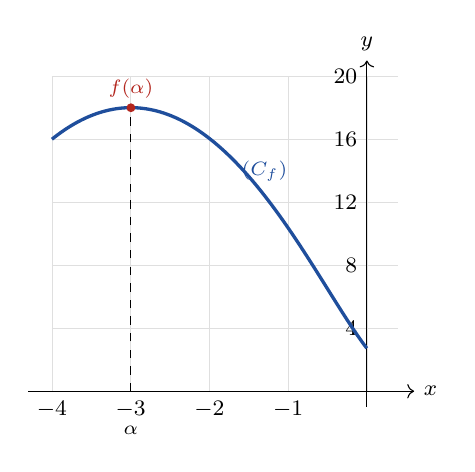
\begin{tikzpicture}[x=1cm,y=0.2cm,font=\footnotesize]
\draw[gray!25,very thin,xstep=1,ystep=4] (-4,0) grid (0.4,20);
\draw[->] (-4.3,0)--(0.6,0) node[right]{$x$}; \draw[->] (0,-1)--(0,21) node[above]{$y$};
\foreach \t in {-4,-3,-2,-1} \node[below] at (\t,0){$\t$};
\foreach \t in {4,8,12,16,20} \node[left] at (0,\t){$\t$};
\draw[cDef,very thick,domain=-4:0,samples=100] plot(\x,{-2*\x*\x-12*\x+exp(2*\x+1)});
\draw[dashed] (-2.997,0)--(-2.997,18.0); \fill[cThm] (-2.997,18.0) circle (1.6pt) node[above,font=\scriptsize]{$f(\alpha)$};
\node[below,font=\scriptsize] at (-2.997,-1.6){$\alpha$};
\node[cDef,font=\scriptsize] at (-1.3,14){$(C_f)$};
\end{tikzpicture}\end{LTR}\par
\QQ{5} $(\star)$ دالة أصلية لـ $f$: $F(x)=-\dfrac23x^3-6x^2+\dfrac12e^{2x+1}$ ، ومنه (مع $e^{2\alpha+1}=2\alpha+6$):
\[\frac12\int_\alpha^0f(x)\,dx=\frac12\left[\frac e2+\frac23\alpha^3+6\alpha^2-\frac12(2\alpha+6)\right]\]
\[\frac12\int_\alpha^0f(x)\,dx=\bx{\frac e4+\frac{\alpha^3}3+3\alpha^2-\frac\alpha2-\frac32}\approx18{,}65\]
\textbf{التفسير:} $f(x)>0$ على $[\alpha;0]$ ، ووحدة المساحة $1\times0{,}5=0{,}5\,cm^2$ ، إذن هذا العدد هو مساحة الحيز المحدد بـ $(C_f)$ ومحور الفواصل والمستقيمين $x=\alpha$ و $x=0$ ، مقدرة بـ $cm^2$.
\end{hal}

\begin{tamrin}{بكالوريا 2018 -- الموضوع الثاني -- التمرين الرابع}
\textbf{I)} نعتبر الدالة العددية $g$ المعرفة على $[0;+\infty[$ بـ: $g(x)=1+(1-x)e^{-x+1}$.\par
ادرس اتجاه تغير الدالة $g$ ثم بيّن أنه من أجل كل $x$ من $[0;+\infty[$: $g(x)>0$ (لا يطلب حساب النهايات).\par
\textbf{II)} نعتبر الدالة العددية $f$ المعرفة على $[0;+\infty[$ بـ: $f(x)=x+xe^{-x+1}$ ، و $(C_f)$ تمثيلها البياني.
\QQ{1}
\begin{sq}
\qa أحسب $\Lm{+\infty}f(x)$ ، ثم بيّن أن المستقيم $(\Delta)$ ذا المعادلة $y=x$ مقارب للمنحنى $(C_f)$.
\qb ادرس وضعية المنحنى $(C_f)$ بالنسبة إلى المستقيم $(\Delta)$.
\end{sq}
\QQ{2} بيّن أنه من أجل كل $x$ من $[0;+\infty[$: $f'(x)=g(x)$ ، ثم شكّل جدول التغيرات للدالة $f$.
\QQ{3} بيّن أن المعادلة $f(x)=4$ تقبل حلًا وحيدًا $\alpha$ حيث: $3{,}75<\alpha<3{,}77$.
\QQ{4} اكتب معادلة المماس $(T)$ للمنحنى $(C_f)$ عند النقطة ذات الفاصلة $1$ ، ثم ارسم $(T)$ ، $(\Delta)$ و $(C_f)$.
\QQ{5} $(\star)$ نعتبر الدالة $F$ المعرفة على $[0;+\infty[$ بـ: $F(x)=\dfrac12x^2-(x+1)e^{-x+1}$.
\begin{sq}
\qa بيّن أن الدالة $F$ هي دالة أصلية للدالة $f$ على المجال $[0;+\infty[$.
\qb أوجد القيمة المضبوطة للعدد $\displaystyle\int_1^4f(x)\,dx$ ، ثم أعط تفسيرًا هندسيًا لهذا العدد.
\end{sq}
\QQ{6} تنمذج الكلفة الهامشية $C_m$ لإنتاج كمية $q$ (مقدرة بآلاف الوحدات) حيث $0\leqslant q\leqslant7$ بالدالة $f$ ، أي: $C_m(q)=f(q)$ (الكلفة الهامشية مقدرة بملايين الدنانير).
\begin{sq}
\qa ما هي كمية المنتوج التي من أجلها لا تتجاوز الكلفة الهامشية $4$ ملايين دينار؟
\qb $(\star)$ نذكّر أن دالة الكلفة الإجمالية $C_T$ هي دالة أصلية لدالة الكلفة الهامشية. أحسب القيمة المتوسطة للكلفة الهامشية عندما تنتج الشركة ما بين $1000$ وحدة و $4000$ وحدة.
\end{sq}
\end{tamrin}
\begin{hal}
\textbf{I)} $g'(x)=-e^{-x+1}+(1-x)(-e^{-x+1})=\bx{(x-2)e^{-x+1}}$ ، إشارتها إشارة $x-2$: $g$ متناقصة تمامًا على $[0;2]$ ومتزايدة تمامًا على $[2;+\infty[$.\par
القيمة الحدية الصغرى: $g(2)=1-e^{-1}>0$ ، إذن $\bx{g(x)>0}$ على $[0;+\infty[$.\par
\textbf{II)}
\QQ{1}
\pa نكتب: $xe^{-x+1}=e\times\dfrac x{e^x}$.
\LD{f(x)}{+\infty}{+\infty} $\Car{\Lm{+\infty}x=+\infty\\[6pt]\Lm{+\infty}e\times\dfrac x{e^x}=0}$\E
$f(x)-x=xe^{-x+1}$ ونهايته عند $+\infty$ هي $0$: \bxt{$(\Delta):\ y=x$ مقارب مائل عند $+\infty$}.
\pb $f(x)-x=xe^{-x+1}\geqslant0$ على $[0;+\infty[$ ، وينعدم عند $0$:
\begin{FIG}
\begin{tikzpicture}[font=\normalsize]
\fill[gray!12] (0,0) rectangle (2.6,-0.9);
\fill[green!18] (2.6,0) rectangle (15,-0.9);
\fill[orange!45] (0,-0.9) rectangle (2.6,-4.6);
\fill[cyan!22] (2.6,-0.9) rectangle (15,-4.6);
\draw[thick] (0,0) rectangle (15,-4.6); \draw (0,-0.9)--(15,-0.9) (0,-1.8)--(15,-1.8) (2.6,0)--(2.6,-4.6);
\node at (1.3,-0.45){$x$};
\node at (1.3,-1.35){$xe^{-x+1}$};
\node[align=center,font=\bfseries] at (1.3,-3.2){\ar{الوضع}\\ \ar{النسبي}};
\node at (4.8,-0.45){$0$};
\node at (14.3,-0.45){$+\infty$};
\node at (10.3,-1.35){$+$};
\node[align=center,font=\small] at (10.3,-3.2){$(C_f)$\\ \ar{فوق}\\ $(\Delta)$};
\node at (4.8,-1.35){$0$};
\draw[densely dotted] (4.8,-0.9)--(4.8,-1.13) (4.8,-1.57)--(4.8,-1.8);
\draw (3.3,-4.6) .. controls (3.375,-3.06) and (4.35,-2.136) .. (4.8,-1.8) .. controls (5.25,-2.136) and (6.225,-3.06) .. (6.3,-4.6);
\node[align=center,font=\footnotesize,inner sep=0pt] at (4.8,-3.65){\ar{$(C_f)$ يقطع}\\ $(\Delta)$\\ \ar{في النقطة}\\ $(0;0)$};
\end{tikzpicture}
\end{FIG}
\QQ{2} $f'(x)=1+e^{-x+1}-xe^{-x+1}=1+(1-x)e^{-x+1}=\bx{g(x)}>0$: \bxt{$f$ متزايدة تمامًا} ، و $f(0)=0$.
\begin{TAB}
\tkzTabInit[lgt=1.6,espcl=4]{$x$/1,$f'(x)$/1,$f(x)$/2}{$0$,$+\infty$}
\tkzTabLine{,+,}
\tkzTabVar{-/$0$,+/$+\infty$}
\end{TAB}
\QQ{3} $f$ مستمرة ومتزايدة تمامًا على $[3{,}75;3{,}77]$ ، و:
\[f(3{,}75)-4\approx-0{,}010<0\qquad;\qquad f(3{,}77)-4\approx0{,}006>0\]
إذن المعادلة $f(x)=4$ تقبل حلًا وحيدًا $\bx{\alpha\in]3{,}75;3{,}77[}$.
\QQ{4} $f(1)=1+1=2$ و $f'(1)=g(1)=1$ ، ومنه $(T)$: $y=(x-1)+2$ ، أي $\bx{(T):\ y=x+1}$.
\begin{GR}{-0.4}{5.6}{-0.5}{5.6}{0.75}
\Ticks{1,2,3,4,5}{1,2,3,4,5}
\draw[cRem!70!black,thick,domain=-0.4:5.6] plot(\x,{\x}) node[below,font=\scriptsize]{$(\Delta)$};
\draw[cThm,thick,domain=-0.4:4.5] plot(\x,{\x+1}) node[above,font=\scriptsize]{$(T)$};
\draw[cDef,very thick,domain=0:5.6,samples=150] plot(\x,{\x+\x*exp(1-\x)});
\node[cDef,font=\scriptsize] at (1.3,3.3){$(C_f)$};
\fill[cThm] (1,2) circle (1.6pt);
\end{GR}
\QQ{5} $(\star)$
\pa $F'(x)=x-\big[e^{-x+1}-(x+1)e^{-x+1}\big]=x+xe^{-x+1}=\bx{f(x)}$.
\pb
\[\int_1^4f(x)\,dx=F(4)-F(1)=\left(8-5e^{-3}\right)-\left(\frac12-2\right)=\bx{\frac{19}2-5e^{-3}}\approx9{,}25\]
\textbf{التفسير:} $f(x)\geqslant0$ على $[1;4]$ ، فهذا العدد هو مساحة الحيز المحدد بـ $(C_f)$ وحامل محور الفواصل والمستقيمين $x=1$ و $x=4$ (بوحدة المساحة).
\QQ{6}
\pa $f$ متزايدة ، إذن $C_m(q)\leqslant4\iff f(q)\leqslant4\iff q\leqslant\alpha$: إذن حتى حوالي \bxt{$3760$ وحدة} ($q\leqslant\alpha\approx3{,}76$).
\pb $(\star)$ القيمة المتوسطة للكلفة الهامشية على $[1;4]$:
\[\frac1{4-1}\int_1^4C_m(q)\,dq=\frac{C_T(4)-C_T(1)}3=\frac{9{,}5-5e^{-3}}3\approx\bx{3{,}08}\ \text{\ar{مليون دينار}}\]
\end{hal}

\begin{tamrin}{بكالوريا 2017 -- الموضوع الثاني -- التمرين الرابع}
نعتبر الدالة $f$ المعرفة على $D_f=]-\infty;0[\cup]0;+\infty[$ كما يلي: $f(x)=\dfrac12e^x-\dfrac1{e^x-1}$ ، و $(C_f)$ تمثيلها البياني.
\QQ{1}
\begin{sq}
\qa أحسب النهايات: $\Lm{-\infty}f(x)$ ، $\Lm{0^-}f(x)$ و $\Lm{0^+}f(x)$ ، وفسّر بيانيًا النتائج المحصل عليها.
\qb أحسب النهاية $\Lm{+\infty}f(x)$.
\end{sq}
\QQ{2}
\begin{sq}
\qa بيّن أنه من أجل كل $x$ من $D_f$: $f'(x)=\dfrac12e^x+\dfrac{e^x}{(e^x-1)^2}$.
\qb استنتج اتجاه تغير الدالة $f$ ثم شكّل جدول تغيراتها.
\end{sq}
\QQ{3} ادرس الوضعية النسبية للمنحنى $(C_f)$ مع المستقيم $(\Delta)$ ذي المعادلة $y=1$.
\QQ{4} عيّن معادلة لـ $(T)$ المماس للمنحنى $(C_f)$ عند النقطة ذات الفاصلة $\ln3$.
\QQ{5} نعتبر الدالة $g$ المعرفة على $]0;+\infty[$ كما يلي: $g(x)=f(x)-\dfrac94(x-\ln3)-1$ ، وهي متزايدة تمامًا من $-\infty$ إلى $+\infty$.
\begin{sq}
\qa أحسب $g(\ln3)$ واستنتج إشارة $g(x)$ حسب قيم $x$.
\qb ادرس على المجال $]0;+\infty[$ وضعية المنحنى $(C_f)$ بالنسبة إلى المماس $(T)$ ، ثم فسّر ذلك بيانيًا.
\end{sq}
\QQ{6} أحسب $f(\ln2)$ ثم ارسم المماس $(T)$ و $(C_f)$ على المجال $]-\infty;0[\cup]0;3]$.
\end{tamrin}
\begin{hal}
\QQ{1}
\pa
\LD{f(x)}{-\infty}{1} $\Car{\Lm{-\infty}\dfrac12e^x=0\\[6pt]\Lm{-\infty}\dfrac1{e^x-1}=\dfrac1{0-1}=-1}$\E
إذن المستقيم $y=1$ مقارب أفقي بجوار $-\infty$.
\LD{f(x)}{0^-}{+\infty} $\Car{\Lm{0^-}\dfrac12e^x=\dfrac12\\[6pt]\Lm{0^-}(e^x-1)=0^-}$\E
لأن $e^x<1$ عندما $x<0$ ، فـ $-\dfrac1{e^x-1}\to+\infty$.
\LD{f(x)}{0^+}{-\infty} $\Car{\Lm{0^+}\dfrac12e^x=\dfrac12\\[6pt]\Lm{0^+}(e^x-1)=0^+}$\E
إذن المستقيم $x=0$ (محور التراتيب) مقارب عمودي.
\pb
\LD{f(x)}{+\infty}{+\infty} $\Car{\Lm{+\infty}\dfrac12e^x=+\infty\\[6pt]\Lm{+\infty}\dfrac1{e^x-1}=0}$\E
\QQ{2}
\pa $\left(\dfrac1{e^x-1}\right)'=-\dfrac{e^x}{(e^x-1)^2}$ ، ومنه $\bx{f'(x)=\dfrac12e^x+\dfrac{e^x}{(e^x-1)^2}}$.
\pb $f'(x)>0$: \bxt{$f$ متزايدة تمامًا على $]-\infty;0[$ وعلى $]0;+\infty[$}.
\begin{TAB}
\tkzTabInit[lgt=1.6,espcl=3]{$x$/1,$f'(x)$/1,$f(x)$/2}{$-\infty$,$0$,$+\infty$}
\tkzTabLine{,+,d,+,}
\tkzTabVar{-/$1$,+D-/$+\infty$/$-\infty$,+/$+\infty$}
\end{TAB}
\QQ{3} نوحد المقامات:
\[f(x)-1=\frac{\frac12e^x(e^x-1)-1-(e^x-1)}{e^x-1}=\frac{\frac12e^{2x}-\frac32e^x}{e^x-1}=\bx{\frac{e^x\left(e^x-3\right)}{2\left(e^x-1\right)}}\]
\begin{TAB}
\tkzTabInit[lgt=2,espcl=2.4]{$x$/1,$e^x-3$/1,$e^x-1$/1,$f(x)-1$/1}{$-\infty$,$0$,$\ln3$,$+\infty$}
\tkzTabLine{,-,t,-,z,+,}
\tkzTabLine{,-,z,+,t,+,}
\tkzTabLine{,+,d,-,z,+,}
\end{TAB}
\begin{FIG}
\begin{tikzpicture}[font=\normalsize]
\fill[gray!12] (0,0) rectangle (2.6,-0.9);
\fill[green!18] (2.6,0) rectangle (15,-0.9);
\fill[orange!45] (0,-0.9) rectangle (2.6,-4.6);
\fill[cyan!22] (2.6,-0.9) rectangle (15,-4.6);
\draw[thick] (0,0) rectangle (15,-4.6); \draw (0,-0.9)--(15,-0.9) (0,-1.8)--(15,-1.8) (2.6,0)--(2.6,-4.6);
\node at (1.3,-0.45){$x$};
\node at (1.3,-1.35){$f(x)-1$};
\node[align=center,font=\bfseries] at (1.3,-3.2){\ar{الوضع}\\ \ar{النسبي}};
\node at (3.3,-0.45){$-\infty$};
\node at (5.88824,-0.45){$0$};
\node at (10.0941,-0.45){$\ln3$};
\node at (14.3,-0.45){$+\infty$};
\node at (4.59412,-1.35){$+$};
\node[align=center,font=\small] at (4.59412,-3.2){$(C_f)$\\ \ar{فوق}\\ $(\Delta)$};
\node at (7.24118,-1.35){$-$};
\node[align=center,font=\small] at (7.24118,-3.2){$(C_f)$\\ \ar{تحت}\\ $(\Delta)$};
\node at (12.9471,-1.35){$+$};
\node[align=center,font=\small] at (12.9471,-3.2){$(C_f)$\\ \ar{فوق}\\ $(\Delta)$};
\draw[double,thick] (5.88824,-0.9)--(5.88824,-4.6);
\node at (10.0941,-1.35){$0$};
\draw[densely dotted] (10.0941,-0.9)--(10.0941,-1.13) (10.0941,-1.57)--(10.0941,-1.8);
\draw (8.59412,-4.6) .. controls (8.66912,-3.06) and (9.64412,-2.136) .. (10.0941,-1.8) .. controls (10.5441,-2.136) and (11.5191,-3.06) .. (11.5941,-4.6);
\node[align=center,font=\footnotesize,inner sep=0pt] at (10.0941,-3.65){\ar{$(C_f)$ يقطع}\\ $(\Delta)$\\ \ar{في النقطة}\\ $(\ln3;1)$};
\end{tikzpicture}
\end{FIG}
\QQ{4} $f(\ln3)=\dfrac32-\dfrac12=1$ و $f'(\ln3)=\dfrac32+\dfrac34=\dfrac94$ ، ومنه $\bx{(T):\ y=\dfrac94(x-\ln3)+1}$.
\QQ{5}
\pa $g(\ln3)=f(\ln3)-0-1=\bx{0}$ ، و $g$ متزايدة تمامًا ، إذن: $g(x)<0$ على $]0;\ln3[$ ، و $g(x)>0$ على $]\ln3;+\infty[$.
\pb $g(x)=f(x)-y_T$: $(C_f)$ تحت $(T)$ على $]0;\ln3[$ وفوقه على $]\ln3;+\infty[$.\par
\textbf{التفسير:} المماس $(T)$ يخترق المنحنى عند النقطة $(\ln3;1)$ ، فهي \bxt{نقطة انعطاف} للمنحنى $(C_f)$.
\QQ{6} $f(\ln2)=\dfrac12\times2-\dfrac1{2-1}=\bx{0}$: المنحنى يقطع محور الفواصل في النقطة $(\ln2;0)$.
\begin{GR}{-3.6}{2.6}{-2.6}{4.6}{0.8}
\Ticks{-3,-2,-1,1,2}{-2,-1,1,2,3,4}
\draw[cRem!70!black,dashed] (-3.6,1)--(2.6,1) node[above left,font=\scriptsize]{$(\Delta)$};
\draw[cThm,thick,domain=0.4:1.85] plot(\x,{2.25*(\x-1.0986)+1}) node[above,font=\scriptsize]{$(T)$};
\draw[cDef,very thick,domain=-3.6:-0.17,samples=120] plot(\x,{0.5*exp(\x)-1/(exp(\x)-1)});
\draw[cDef,very thick,domain=0.2:1.9,samples=120] plot(\x,{0.5*exp(\x)-1/(exp(\x)-1)});
\fill[cThm] (1.0986,1) circle (1.6pt);
\node[cDef,font=\scriptsize] at (-2.6,1.6){$(C_f)$};
\end{GR}
\end{hal}

\begin{tamrin}{بكالوريا 2017 (الدورة الاستثنائية) -- الموضوع الأول -- التمرين الرابع}
\textbf{I)} لتكن $g$ الدالة المعرفة على $\R$ كما يلي: $g(x)=2x-1-e^{2x}$.
\QQ{1} ادرس اتجاه تغير الدالة $g$.
\QQ{2} استنتج إشارة $g(x)$.\par
\textbf{II)} نعتبر الدالة $f$ المعرفة على $\R$ كما يلي: $f(x)=x^2-x-\dfrac12e^{2x}$ ، و $(C_f)$ تمثيلها البياني ($\|\vec i\|=2\,cm$).
\QQ{1} أحسب $\Lm{-\infty}f(x)$ و $\Lm{+\infty}f(x)$. (يعطى: $\Lm{+\infty}\dfrac{e^{2x}}{x^2}=+\infty$).
\QQ{2} ادرس اتجاه تغير الدالة $f$ ثم شكّل جدول تغيراتها.
\QQ{3}
\begin{sq}
\qa بيّن أن المعادلة $f(x)=0$ تقبل حلًا وحيدًا $\alpha$ حيث $-0{,}25<\alpha<-0{,}24$.
\qb أثبت أن المنحنى $(C_f)$ يقبل نقطة انعطاف $A$ إحداثياها $\left(0;-\dfrac12\right)$.
\qc اكتب معادلة المماس $(T)$ للمنحنى $(C_f)$ في النقطة $A$.
\end{sq}
\QQ{4} ارسم $(T)$ و $(C_f)$.
\QQ{5} $(\star)$
\begin{sq}
\qa أحسب بالسنتيمتر المربع المساحة $A(\alpha)$ للحيز المحدد بالمنحنى $(C_f)$ والمستقيمات التي معادلاتها $y=0$ ، $x=\alpha$ و $x=0$.
\qb تحقق أن $A(\alpha)=\dfrac13\left(4\alpha^3-12\alpha^2+6\alpha+3\right)cm^2$.
\end{sq}
\end{tamrin}
\begin{hal}
\textbf{I)}
\QQ{1} $g'(x)=2-2e^{2x}$ ؛ $g'(x)=0\iff e^{2x}=1\iff x=0$ ؛ $g'(x)>0\iff x<0$.\par
\bxt{$g$ متزايدة تمامًا على $]-\infty;0]$ ومتناقصة تمامًا على $[0;+\infty[$} ، وقيمتها الحدية العظمى $g(0)=-1-1=-2$.
\QQ{2} بما أن القيمة العظمى $g(0)=-2<0$ ، فإن من أجل كل $x\in\R$: $\bx{g(x)<0}$.\par
\textbf{II)}
\QQ{1}
\LD{f(x)}{-\infty}{+\infty} $\Car{\Lm{-\infty}(x^2-x)=+\infty\\[6pt]\Lm{-\infty}\dfrac12e^{2x}=0}$\E
عند $+\infty$ حالة عدم تعيين ، نكتب: $f(x)=x^2\left(1-\dfrac1x-\dfrac12\times\dfrac{e^{2x}}{x^2}\right)$.
\LD{f(x)}{+\infty}{-\infty} $\Car{\Lm{+\infty}x^2=+\infty\\[6pt]\Lm{+\infty}\left(1-\dfrac1x-\dfrac12\times\dfrac{e^{2x}}{x^2}\right)=-\infty}$\E
\QQ{2} $f'(x)=2x-1-\dfrac12\times2e^{2x}=2x-1-e^{2x}=\bx{g(x)}<0$: \bxt{$f$ متناقصة تمامًا على $\R$}.
\begin{TAB}
\tkzTabInit[lgt=1.6,espcl=4]{$x$/1,$f'(x)$/1,$f(x)$/2}{$-\infty$,$+\infty$}
\tkzTabLine{,-,}
\tkzTabVar{+/$+\infty$,-/$-\infty$}
\end{TAB}
\QQ{3}
\pa $f$ مستمرة ومتناقصة تمامًا ، و:
\[f(-0{,}25)\approx0{,}009>0\qquad;\qquad f(-0{,}24)\approx-0{,}012<0\]
إذن المعادلة $f(x)=0$ تقبل حلًا وحيدًا $\bx{\alpha\in]-0{,}25;-0{,}24[}$.
\pb $f''(x)=g'(x)=2-2e^{2x}$ تنعدم عند $0$ وتغير إشارتها (موجبة قبل $0$ وسالبة بعده) ، و $f(0)=-\dfrac12$: \bxt{$A\left(0;-\frac12\right)$ نقطة انعطاف}.
\pc $f'(0)=g(0)=-2$ ، ومنه $\bx{(T):\ y=-2x-\dfrac12}$.
\QQ{4} الرسم ($\|\vec i\|=2\,cm$):
\begin{GR}{-1.6}{1.4}{-2.6}{3.8}{1}
\Ticks{-1,1}{-2,-1,1,2,3}
\draw[cThm,thick,domain=-1.6:1.05] plot(\x,{-2*\x-0.5}) node[right,font=\scriptsize]{$(T)$};
\draw[cDef,very thick,domain=-1.6:1.1,samples=150] plot(\x,{\x*\x-\x-0.5*exp(2*\x)});
\fill[cThm] (0,-0.5) circle (1.6pt) node[right,font=\scriptsize]{$A$};
\node[cDef,font=\scriptsize] at (-1.2,3.4){$(C_f)$};
\end{GR}
\QQ{5} $(\star)$
\pa على $[\alpha;0]$: $f$ متناقصة و $f(\alpha)=0$ ، إذن $f(x)\leqslant0$. دالة أصلية: $F(x)=\dfrac{x^3}3-\dfrac{x^2}2-\dfrac14e^{2x}$. ووحدة المساحة $4\,cm^2$:
\[A(\alpha)=-4\int_\alpha^0f(x)\,dx=-4\left[-\frac14-\frac{\alpha^3}3+\frac{\alpha^2}2+\frac14e^{2\alpha}\right]=1+\frac43\alpha^3-2\alpha^2-e^{2\alpha}\]
\pb $f(\alpha)=0$ معناه $\dfrac12e^{2\alpha}=\alpha^2-\alpha$ ، أي $e^{2\alpha}=2\alpha^2-2\alpha$ ، ومنه:
\[A(\alpha)=1+\frac43\alpha^3-2\alpha^2-2\alpha^2+2\alpha=\bx{\frac13\left(4\alpha^3-12\alpha^2+6\alpha+3\right)cm^2}\approx0{,}25\,cm^2\]
\end{hal}

% =====================================================
\section{أسئلة الاختيار من متعدد (من البكالوريا والاختبارات)}
\begin{tamrin}{عيّن الاقتراح الصحيح الوحيد من بين الاقتراحات الثلاثة مع التبرير}
\QQ{1} (بكالوريا 2026) النهاية $\Lm{-\infty}\left(\dfrac{e^x-1}{e^x+1}\right)$ تساوي:\ABC{$-1$}{$1$}{$+\infty$}
\QQ{2} (بكالوريا 2026) مجموعة حلول المتراجحة $e^{-x}-e^2\geqslant0$ في $\R$ هي:\ABC{$]-\infty;-2]$}{$[-2;2]$}{$[-2;+\infty[$}
\QQ{3} (بكالوريا 2026) الدالة المشتقة للدالة $f(x)=(1-x)e^x$ هي:\ABC{$f'(x)=1-xe^x$}{$f'(x)=(1-2x)e^x$}{$f'(x)=-xe^x$}
\QQ{4} (بكالوريا 2026) $(c_k)$ منحنى الدالة $k(x)=e^{1-x}$ ، والمستقيم $(T):\ y=-x+2$ مماس لـ $(c_k)$ في النقطة $A$ ذات الفاصلة $x_0$ حيث:\ABC{$x_0=1$}{$x_0=0$}{$x_0=-1$}
\QQ{5} (بكالوريا 2025) مجموعة حلول المعادلة $1-3e^{-x}=0$ في $\R$ هي:\ABC{$\{-\ln3\}$}{$\left\{\dfrac13\right\}$}{$\{\ln3\}$}
\QQ{6} (بكالوريا 2024) المعادلة $2e^{2x}+3e^x-2=0$ ذات المجهول الحقيقي $x$:\ABC{تقبل حلًا وحيدًا}{تقبل حلين مختلفين}{لا تقبل حلولًا}
\QQ{7} $(\star)$ (بكالوريا 2024) $\displaystyle\int_0^1\left(3x^2+3e^{3x}\right)dx$ يساوي:\ABC{$e^3+1$}{$e^3$}{$e^3-1$}
\QQ{8} (بكالوريا 2023) مجموعة الحلول في $\R$ للمعادلة $e^{2x}+4e^x-5=0$ هي:\ABC{$\{0\}$}{$\{1;0\}$}{$\{-5;0\}$}
\QQ{9} (بكالوريا 2023) $\Lm{+\infty}\left(x+1-e^x\right)$ تساوي:\ABC{$-\infty$}{$+\infty$}{$0$}
\QQ{10} (بكالوريا تجريبية 2026) مجموعة حلول المعادلة $1-4e^{-2x}=0$ في $\R$ هي:\ABC{$\{\ln2\}$}{$\{-\ln2\}$}{$\left\{-\dfrac18\right\}$}
\QQ{11} (بكالوريا تجريبية 2025) $f(x)=\dfrac{e^x-2}{2e^x+1}$ ، النهاية $\Lm{-\infty}f(x)$ هي:\ABC{$-2$}{$2$}{$\dfrac12$}
\QQ{12} $(\star)$ (بكالوريا تجريبية 2025) القيمة المتوسطة للدالة $f(x)=xe^{-x}$ على المجال $[0;1]$ هي:\ABC{$1-\dfrac2e$}{$\dfrac1e$}{$1-\dfrac1e$}
\end{tamrin}
\begin{hal}
\QQ{1} $\Lm{-\infty}e^x=0$ ، ومنه النهاية $\dfrac{0-1}{0+1}=-1$. \quad \bxt{الجواب (أ)}.
\QQ{2} $e^{-x}\geqslant e^2\iff-x\geqslant2\iff x\leqslant-2$. \quad \bxt{الجواب (أ)}.
\QQ{3} $f'(x)=-e^x+(1-x)e^x=-xe^x$. \quad \bxt{الجواب (جـ)}.
\QQ{4} $k'(x)=-e^{1-x}$. معامل توجيه المماس $-1$: $-e^{1-x_0}=-1\iff x_0=1$ ، وفعلًا $k(1)=1=-1+2$. \quad \bxt{الجواب (أ)}.
\QQ{5} $3e^{-x}=1\iff e^{-x}=\dfrac13\iff-x=-\ln3\iff x=\ln3$. \quad \bxt{الجواب (جـ)}.
\QQ{6} نضع $X=e^x>0$: $2X^2+3X-2=0$ ، $\Delta=25$ ، $X=\dfrac12$ أو $X=-2$ (مرفوض) ، ومنه حل وحيد $x=-\ln2$. \quad \bxt{الجواب (أ)}.
\QQ{7} $\Big[x^3+e^{3x}\Big]_0^1=(1+e^3)-(0+1)=e^3$. \quad \bxt{الجواب (ب)}.
\QQ{8} $X=e^x$: $X^2+4X-5=(X-1)(X+5)=0$ ، $X=1$ ($X=-5$ مرفوض) ، ومنه $x=0$. \quad \bxt{الجواب (أ)}.
\QQ{9} نكتب: $x+1-e^x=x\left(1+\dfrac1x-\dfrac{e^x}x\right)$.
\par لدينا: $\Lm{+\infty}(x+1-e^x)=\bx{-\infty}$ لأنّ: \quad $\Car{\Lm{+\infty}x=+\infty\\[6pt]\Lm{+\infty}\left(1+\dfrac1x-\dfrac{e^x}x\right)=-\infty}$\E
\bxt{الجواب (أ)}.
\QQ{10} $e^{-2x}=\dfrac14\iff e^{2x}=4\iff2x=\ln4=2\ln2\iff x=\ln2$. \quad \bxt{الجواب (أ)}.
\QQ{11} $\Lm{-\infty}e^x=0$: النهاية $\dfrac{0-2}{0+1}=-2$. \quad \bxt{الجواب (أ)}.
\QQ{12} دالة أصلية لـ $xe^{-x}$ هي $-(x+1)e^{-x}$ ، ومنه $m=\dfrac1{1-0}\Big[-(x+1)e^{-x}\Big]_0^1=-2e^{-1}+1$. \quad \bxt{الجواب (أ)}.
\end{hal}

\begin{BOX}{cSec}{}
\centering{\Large\bfseries بالتوفيق في شهادة البكالوريا}
\end{BOX}
\end{document}
